% !TeX root = ../../book.tex
\chapter[数学归纳法]{数学归纳法:``依此类推''}\label{ch:chapter02}

% !TeX root = ../../../book.tex
\section{引言}

本章旨在深入探讨数学证明方法,并引导读者学习如何自行构建数学证明。我们首次引入一种重要的\textbf{证明技术},即\textbf{数学归纳法}。本章作为初步介绍,旨在帮助读者建立对该方法的基本认知。后续章节将严格定义归纳法并\emph{证明}其数学合理性——我们将深入探讨其原理与有效性。现在,让我们通过精选的范例问题,体验归纳法的实际应用。

% !TeX root = ../../../book.tex
\subsection{目标}

以下简要说明本章在本书中的定位:它将阐释先前内容如何发挥作用,阐述研究本章主题的动机,明确学习目标,并提示阅读时的关注重点。我们先列出本章的核心目标及学成后应掌握的技能,后续章节将详细展开。学完本章后,请返回此处核验:你是否理解所有目标?能否阐述其重要性?能否定义相关术语?能否运用相关技术?

\textbf{学完本章后,你应该能够……}

\begin{itemize}
    \item 明确数学归纳法的定义,并对给定证明方法进行归纳法/非归纳法分类
    \item 根据问题特征判断适用归纳法的场景
    \item 通过类比方式直观描述数学归纳法的运作机制
    \item 辨别不同归纳证明的异同,分析其对应问题的结构特征
\end{itemize}


% !TeX root = ../../../book.tex
\subsection{承上}

与上一章一样,我们假设你只熟悉基本代数和算术,以及视觉、几何直觉,对除此之外的更高等的数学知之甚少。但我们会频繁使用求和和求积符号,因此,如果你觉得自己的符号技能有所欠缺,请回看第 \ref{sec:section1.3.5} 节。


% !TeX root = ../../../book.tex
\subsection{启下}

回顾 \ref{sec:section1.4.3} 节的问题,我们证明了前 $n$ 个奇数之和等于 $n^2$。最初通过几何视角观察这一模式:将奇数项排列为逐渐扩大的正方形``角块''。然而,第一种证明方法似乎并未依赖这一观察,而是以\emph{代数}方式运用了关于偶数与奇数之和的既有结论——通过对若干等式进行乘法、减法等操作,最终得到了预期结果。这种方法是否令人满意?它在某种程度上偏离了最初的几何解释,其有效性或许出人意料。(也许存在\emph{不同的}几何解释?读者可尝试探寻。)

第二种方法则是对几何观察的代数建模。我们将求和与正方形面积建立联系,将求和项对应于图形的特定部分。通过在不同问题解释间构建\emph{对应关系},使几何与代数解释互为支撑,共同指向同一结论。这种视觉化优势在于启发了名为\textbf{数学归纳法}的通用证明策略(简称\textbf{归纳法})。(请注意:\emph{归纳法}在电磁学或哲学等领域另有含义,但本书特指\emph{数学归纳法}。)究竟何为归纳法?其运作机制如何?适用范围是什么?如何针对具体问题调整策略?是否存在更有效的变体?本章将解答这些问题。

首先要探讨的,是此前未提及的核心问题:``\emph{为何}采用归纳法?\emph{为何}重视它?''基于 \ref{sec:section1.4.3} 节的问题,数学归纳法看似并非必需,因为其他方法同样可完成证明。这在一定背景下成立,但需强调:\emph{归纳法极具实用价值!}在众多情形中,它是最简洁的证明途径,且作为通用策略可广泛应用于同类问题。此外,适用归纳法的问题需具备特定\text{结构}——即结果的``后续部分''依赖``前序部分''。(``部分''与``依赖''的具体含义取决于上下文。)识别归纳法的适用性并完成证明过程,常能揭示问题的内在结构。即使归纳证明失败,发现``破坏''归纳步骤的具体环节,往往也能提供深刻洞见。

我们将通过若干示例阐明这些观点,再给出数学归纳法的完整\emph{定义}以展示其通用原理。(\text{严格}的形式化定义将延后至后续章节,待集合论、逻辑陈述与蕴涵等基础概念完备后展开。目前给出的定义已足以解决一些有趣的难题,并支撑归纳法作为通用证明策略的讨论。)


% !TeX root = ../../../book.tex
\subsection{忠告}

请注意,我们仍在朝着数学严谨的目标迈进,或者说在本书和课程的范围与时间安排内尽可能地实现这一目标。我们在本章中提出的一些主张将在稍后得到澄清并在技术上得到证明,这需要自然数和一些基本数理逻辑为基础。一切都有恰当的安排!

尽管如此,本章仍然非常重要,因为我们将继续介绍解决数学问题的过程,应用我们现有的知识和技术来发现新事实并向他人做出解释。 此外,数学归纳法是一种基本的证明技术,很可能会出现在所有其他数学课程中!这是因为它的实用性以及归纳性质在整个数学世界中的普遍性决定的。

\newpage
% !TeX root = ../../../book.tex
\section{案例研讨}

% !TeX root = ../../../book.tex
\subsection{构建更大的立方体}

为了引出数学归纳法的整体方法,让我们看一道几何题并一起解决它。这个例子是精心挑选出来的,旨在说明当问题具有特定类型的结构时,数学归纳法如何与之关联;具体来说就是,某些真理、事实或洞察\emph{取决于}、\emph{依赖于}或可以从``先前的''事实\emph{推导}得出。这种对先前案例(或多个案例)的依赖使得过程具有\emph{归纳性},当我们观察到这种现象时,应用\emph{归纳法}几乎总是一个好主意。

\subsubsection*{$1$ 阶立方体到 $2$ 阶立方体}

让我们来考察一下立方数,尤其是,让我们试着用前一个立方数来描述一个立方数。想象一个 $1 \times 1 \times 1$ 的立方体,让它作为单位块。我们如何通过添加 $1 \times 1 \times 1$ 的块来构建尺寸为 $2 \times 2 \times 2$ 的``下一个最大''立方体?我们需要添加多少个?从算术上讲,我们知道答案:$2^3 = 8$ 且 $1^3 = 1$,因此我们需要添加 $7$ 个块才能得到正确的体积。好吧,这是一个具体的答案,但它并没有完全告诉我们如何排列这 $7$ 个块来构成一个立方体,也没有让我们深入了解如何回答构建\emph{更大}立方体这个问题。最终,我们想回答的是,需要多少块才能从 $100 \times 100 \times 100$ 的立方体构建出 $101 \times 101 \times 101$ 的立方体,而无需执行大量繁琐的计算;也就是说,我们希望最终找到问题的答案:给定一个 $n \times n \times n$ 的立方体,我们需要添加多少块才能将其构建为 $(n+ 1) \times (n+ 1) \times (n+ 1)$ 的立方体?考虑到这一点,让我们仔细思考这个最初的案例,并尝试用一般性的论点来回答它。

给定一个单位块,并且我们知道必须向其添加 $7$ 个块,让我们试着确定这 $7$ 个块应该放置在哪里,以形成 $2 \times 2 \times 2$ 的立方体。(为了简单起见,对于 $n$ 的任意值,我们把大小为 $n \times n \times n$ 的立方体称为 $n$ 阶立方体。在这个例子中,$n$ 的值只取自然数,即非负整数。)查看下面 $1$ 阶立方体和 $2$ 阶立方体的图片,并试着解释如何从一个立方体构建另一个立方体。

\begin{center}
    \begin{tikzpicture}
        \pic {annotated cuboid};

        \foreach \x in {0,1}
            \foreach \y in {0,1}
                \foreach \z in {0,1}
                    \pic [fill=white] at (4+\x,\y,\z) {annotated cuboid};
        % \pic [very thick,densely dashed,draw=blue] at (5,0) {annotated cuboid={width=30, height=5, depth=10, opacity=0.2}};
    \end{tikzpicture}
\end{center}

这是我们想要使用的一个合理的解释,因为它能指导我们给出从 $n$ 阶立方体构建 $(n+1)$ 阶立方体的一般解释,并且它是一种数学上优雅且简单的解释。从上面的 $1$ 阶立方体开始,将 $3$ 个暴露的面``放大''适当的量,在本例中为 $1$ 块。到目前为止,这占 $7$ 个块中的 $3$ 个:$2^3 = 1^3+3+\underline{\qquad}$。现在还缺哪里?

\begin{center}
    \begin{tikzpicture}
        \pic {annotated cuboid};
        \pic at (1,-1,0) {annotated cuboid};
        \pic at (0,-1,1) {annotated cuboid};
    \end{tikzpicture}
\end{center}

我们刚刚添加的块在每对块之间都产生了``间隙'',并且每个``间隙''都可以用一个块填充。这占了 $7$ 个块中的 $3$ 个:$2^3 = 1^3+3+3+\underline{\qquad}$。接下来呢?

\begin{center}
    \begin{tikzpicture}
        \pic {annotated cuboid};
        \foreach \x in {0,1}
            \foreach \y in {0,1}
                    \pic [fill=white] at (\x,\y,0) {annotated cuboid};
        \pic [fill=white] at (0,0,1) {annotated cuboid};
        \pic [fill=white] at (0,1,1) {annotated cuboid};
        \pic [fill=white] at (1,0,1) {annotated cuboid};
        % \pic [very thick,densely dashed,draw=blue] at (5,0) {annotated cuboid={width=30, height=5, depth=10, opacity=0.2}};
    \end{tikzpicture}
\end{center}

只剩下一个块需要填充,位于最顶角。添加这个块就完成了 $2$ 阶立方体的构建,并且我们还得到了如何使用以下图形和方程以数学的方式描述我们的构建过程:

\begin{center}
    \begin{tikzpicture}
        \pic {annotated cuboid};

        \pic [densely dashed] at (3, 0) {annotated cuboid};
        \pic [very thick,draw=blue] at (4.2,0,0) {annotated cuboid};
        \pic [very thick,draw=blue] at (3,1.2,0) {annotated cuboid};
        \pic [very thick,draw=blue] at (3,0,1.4) {annotated cuboid};

        \pic [densely dashed] at (7.5,1,0) {annotated cuboid};
        \pic [densely dashed] at (8.5,0,0) {annotated cuboid};
        \pic [densely dashed] at (7.5,0,1) {annotated cuboid};
        \pic [very thick,draw=red] at (8.7,1.2,-0.1) {annotated cuboid};
        \pic [very thick,draw=red] at (7.3,1,1.4) {annotated cuboid};
        \pic [very thick,draw=red] at (8.7,-0.2,1) {annotated cuboid};

        \foreach \x in {0,1}
            \foreach \y in {0,1}
                \pic [densely dashed, fill=white] at (12+\x,\y,0) {annotated cuboid};
        \pic [densely dashed, fill=white] at (12,0,1) {annotated cuboid};
        \pic [densely dashed, fill=white] at (12,1,1) {annotated cuboid};
        \pic [densely dashed, fill=white] at (13,0,1) {annotated cuboid};
        \pic [very thick,draw=olivegreen] at (13.3,1,1.4) {annotated cuboid};
    \end{tikzpicture}
\end{center}

\begin{center}
    \large $2^3 = 1^3+\textcolor{blue}{3}+\textcolor{red}{3}+\textcolor{olivegreen}{1}$
\end{center}

\subsubsection*{$2$ 阶立方体到 $3$ 阶立方体}

现在我们可能对如何描述这个过程有了更好的了解,但让我们多考察两个案例,以确保我们有完整的想法。

让我们从 $2$ 阶立方体开始,构造一个 $3$ 阶立方体。(如果碰巧你手上有各种尺寸的魔方,你甚至可以手动尝试一下!)我们可以遵循与上一个案例类似的步骤,只需适当更改数字即可。从相似的图形开始

\begin{center}
    \begin{tikzpicture}[scale=1]
        \pic {annotated cuboid};
        \foreach \x in {0,1}
            \foreach \y in {0,1}
                \foreach \z in {0,1}
                    \pic [fill=white] at (\x,\y,\z) {annotated cuboid};
        \foreach \x in {0,1,2}
            \foreach \y in {0,1,2}
                \foreach \z in {0,1,2}
                    \pic [fill=white] at (\x+4,\y,\z) {annotated cuboid};
    \end{tikzpicture}
\end{center}

可见我们需要``放大'' $2$ 阶立方体的三个暴露面,但在这种情况下,我们需要放大的量与以前($1$ 阶立方体)\emph{不同},因为我们现在使用的是更大的初始立方体。具体来说,每个面必须放大 $2 \times 2$ 的\emph{正方形}块(而在之前的情况下,我们添加了 $1 \times 1$ 的正方形块)因此,此添加过程的方程是
\[3^2 = 2^3+3\cdot2^2+\underline{\qquad}\]

\begin{center}
    \begin{tikzpicture}[scale=1]
        \foreach \x in {0,1}
            \foreach \y in {0,1}
                \pic [fill=white] at (\x,\y,2) {annotated cuboid};
        \foreach \x in {0,1}
            \foreach \z in {0,1}
                \pic [fill=white] at (\x,2,\z) {annotated cuboid};
        \foreach \y in {0,1}
            \foreach \z in {0,1}
                \pic [fill=white] at (2,\y,\z) {annotated cuboid};
    \end{tikzpicture}
\end{center}

这样做之后,我们发现需要使用 $2 \times 1$ 的块来填充这些放大的面之间的间隙(而在之前的情况下,我们添加了 $1 \times 1$ 的块)。到目前为止,添加过程的方程是
\[3^2 = 2^3+3\cdot2^2+3\cdot2+\underline{\qquad}\]

\begin{center}
    \begin{tikzpicture}[scale=1]
        \foreach \x in {0,1,2}
            \foreach \y in {0,1,2}
                \foreach \z in {0,1}
                    \pic [fill=white] at (\x,\y,\z) {annotated cuboid};
        \foreach \x in {0,1}
            \foreach \y in {0,1,2}
                \pic [fill=white] at (\x,\y,2) {annotated cuboid};
        \foreach \y in {0,1}
            \pic [fill=white] at (2,\y,2) {annotated cuboid};
    \end{tikzpicture}
\end{center}

这样做之后,我们看到只剩下顶角需要填充。因此,我们可以描述我们的构建过程及其相应的方程:

\begin{center}
    \begin{tikzpicture}[scale=1]
        \foreach \x in {0,1}
            \foreach \y in {0,1}
                \foreach \z in {0,1}
                    \pic [very thick, fill=white] at (\x,\y,\z) {annotated cuboid};

        \foreach \x in {0,1}
            \foreach \y in {0,1}
                \foreach \z in {0,1}
                    \pic [densely dashed, fill=white] at (\x+6,\y,\z) {annotated cuboid};
        \foreach \x in {0,1}
            \foreach \y in {0,1}
                \pic [very thick,fill=white,draw=blue] at (\x+6,\y,2.4) {annotated cuboid};
        \foreach \x in {0,1}
            \foreach \z in {0,1}
                \pic [very thick,fill=white,draw=blue] at (\x+6,2.3,\z) {annotated cuboid};
        \foreach \y in {0,1}
            \foreach \z in {0,1}
                \pic [very thick,fill=white,draw=blue] at (8.3,\y,\z) {annotated cuboid};

        \foreach \x in {0,1}
            \foreach \y in {0,1}
                \pic [densely dashed,fill=white] at (\x,\y-5,2) {annotated cuboid};
        \foreach \x in {0,1}
            \foreach \z in {0,1}
                \pic [densely dashed,fill=white] at (\x,-3,\z) {annotated cuboid};
        \foreach \y in {0,1}
            \foreach \z in {0,1}
                \pic [densely dashed,fill=white] at (2,\y-5,\z) {annotated cuboid};
        \foreach \x in {0,1}
            \pic [very thick,draw=red,fill=white] at (\x-0.3,-3,2.4) {annotated cuboid};
        \foreach \y in {0,1}
            \pic [very thick,draw=red,fill=white] at (2.3,\y-5,2.4) {annotated cuboid};
        \foreach \z in {0,1}
            \pic [very thick,draw=red,fill=white] at (2.3,-3,\z-0.4) {annotated cuboid};

        \foreach \x in {0,1,2}
            \foreach \y in {0,1,2}
                \foreach \z in {0,1}
                    \pic [densely dashed,fill=white] at (\x+6,\y-5,\z) {annotated cuboid};
        \foreach \x in {0,1}
            \foreach \y in {0,1,2}
                \pic [densely dashed,fill=white] at (\x+6,\y-5,2) {annotated cuboid};
        \foreach \y in {0,1}
            \pic [densely dashed,fill=white] at (8,\y-5,2) {annotated cuboid};
        \pic [very thick,draw=olivegreen] at (8.3,-3,2.4) {annotated cuboid};
    \end{tikzpicture}
\end{center}

\begin{center}
    \large $3^3 = 2^3+\textcolor{blue}{3 \cdot 2^2}+\textcolor{red}{3 \cdot 2}+\textcolor{olivegreen}{1}$
\end{center}

\subsubsection*{$n$ 阶立方体到 $n+1$ 阶立方体}

你知道这个过程如何泛化吗?如果我们从 $n$ 阶立方体开始怎么办?我们如何构造一个 $(n + 1)$ 阶立方体?我们按照前两个案例中使用的相同步骤进行操作。首先,我们通过添加三个\emph{正方形}块来放大三个暴露面。每个正方形块有多大?我们希望每个正方形块的大小与暴露面的大小相同,因此它们是 $n \times n$ 的正方形块,每个面有 $n^2$ 个单位块:

\begin{center}
    \begin{tikzpicture}[scale=0.20]
        \pic [densely dashed] {annotated cuboid={width=30, height=30, depth=30}};
        \pic at (2,0,0) {annotated cuboid={width=2, height=30, depth=30}};
        \pic at (0,2,0) {annotated cuboid={width=30, height=2, depth=30}};
        \pic at (0,0,3.6) {annotated cuboid={width=30, height=30, depth=3}};
    \end{tikzpicture}
\end{center}

\[(n+1)^3 = n^3+3n^2+\underline{\qquad}\]

接下来,我们要用行块填充这些放大面之间的间隙。这些行有多长?它们都位于我们刚刚添加的正方形块的边缘,因此它们的大小均为 $n \times 1$,每个间隙有 $n$ 个块:

\begin{center}
    \begin{tikzpicture}[scale=0.20]
        \pic [densely dashed] {annotated cuboid={width=30, height=30, depth=30}};
        \pic [densely dashed,fill=white] at (1,0,0) {annotated cuboid={width=2, height=30, depth=30}};
        \pic [densely dashed,fill=white] at (0,1,0) {annotated cuboid={width=30, height=2, depth=30}};
        \pic [densely dashed,fill=white] at (0,0,1) {annotated cuboid={width=30, height=30, depth=3}};
        \pic at (1,2,3.6) {annotated cuboid={width=30, height=2, depth=3}};
        \pic at (2,1,3.6) {annotated cuboid={width=2, height=30, depth=3}};
        \pic at (2.2,2,2.25) {annotated cuboid={width=2, height=2, depth=30}};
    \end{tikzpicture}
\end{center}

\[(n+1)^3 = n^3+3n^2+3n+\underline{\qquad}\]

最后就只剩下顶角需要填充了!所以,

\[(n+1)^3 = n^3+3n^2+3n+1\]

``等一下!'' 你可能会说,``我们早就知道这个结果了。'' 某种程度上,是的;上面的等式是一个代数恒等式,我们也可以通过展开左侧的乘积再合并同类项轻松得到它:

\begin{align*}
    (n + 1)^3 &= (n + 1) \cdot (n + 1)^2\\
    &= (n + 1) \cdot (n^2 + 2n + 1)\\
    &= (n^3 + 2n^2 + n) + (n^2 + 2n + 1) \\
    &= n^3 + 3n^2 + 3n + 1
\end{align*}

那么我们真正取得了什么成果呢?其实,以几何和视觉方式推导出这个恒等式其背后的要点是,它展示了这个恒等式如何表示某种\emph{归纳}过程。我们试图解释如何从先前已知的``事实''(下一个最小立方数,$n^3$)推导出该``事实''(立方数,$(n + 1)^3$),并正确解释如何做到这一点。将此与我们研究奇数之和为完全平方数时使用的方法进行比较。我们对技术之和的观察也隐含了一个归纳过程,尽管我们当时没有这样描述,但我们鼓励你现在思考一下这个问题。回顾一下我们之前的讨论,并尝试通过查看正方形块来写出如何用 $n^2$ 来写出 $(n + 1)^2$。它看起来像``明显的''代数恒等式吗?(如果你雄心勃勃,想一想用 $n^4$ 来写出 $(n + 1)^4$ 会发生什么。这背后有任何几何直觉吗?更高次幂呢?)

这种方法的好处是,我们知道如何用更小的立方数(一直到 $1$)来描述一个立方数;也就是说,每当我们在表达式中看到立方数时,我们都知道如何用更小的立方数和一些剩余项来写出该值。此外,这些表达式和剩余项中的每一个都具有某种固有结构,取决于具体讨论的立方数。因此,通过我们上面导出的表达式迭代地替换任意立方数(例如 $(n + 1)^3$),持续进行下去直到无法再替换为止,应该会产生一个具有一定内在对称性的方程。这个想法最好通过实际行动来说明,所以让我们看看会发生什么。让我们从之前推导出的表达式开始,对于 $n$ 的某个任意值,

\[(n+1)^3 = n^3+3n^2+3n+1\]

接着我们就知道一个类似的表达

\[n^3 = (n-1)^3+3(n-1)^2+3(n-1)+1\]

当我们给出 $n^3$ 的上述表达式的一般论证时,我们证明了这个方程成立,因为这仅依赖于 $n \ge 1$ 的事实。我们可以遵循相同的逻辑步骤,在整个过程中将 $n$ 替换为 $n - 1$,并最终得到上面第二个表达式,也就是 $(n - 1)^3$ 的表达式。(对于 $n$ 的任意值,这种情况都会继续下去吗?思考一下。当 $n \le 0$ 时,我们的论证有意义吗?比如说,从不同的立方体构造 $(-2) \times (- 2) \times (-2)$ 的立方体,这在物理上有意义吗?)

因此,我们可以替换上面一行中的 $n^3$ 项

\begin{center}
    \begin{tabular}{rcccccccc}
        $(n+1)^3=$ &     & $\cancel{n^3}$ & $+$ &   $3n^2$   & $+$ &   $3n$   & $+$ & $1$\\
                   & $+$ & $(n-1)^3$      & $+$ & $3(n-1)^2$ & $+$ & $3(n-1)$ & $+$ & $1$\\
    \end{tabular}
\end{center}

这也是一个代数恒等式,但我们肯定不会轻易地想到通过展开左侧的乘积并合并同类项来写出这个恒等式。这里,我们一遍又一遍地利用结果的结构,并得到我们原本不会想到的新表达式。让我们继续这个替换过程,看看它会带我们去到哪里!接下来,我们将 $(n - 1)^3$ 替换为相应的表达式,并得到

\begin{center}
    \begin{tabular}{rcccccccc}
        $(n+1)^3=$ &     &                    &     &   $3n^2$   & $+$ &   $3n$   & $+$ & $1$\\
                   &     & $\cancel{(n-1)^3}$ & $+$ & $3(n-1)^2$ & $+$ & $3(n-1)$ & $+$ & $1$\\
                   & $+$ & $(n-2)^3$          & $+$ & $3(n-2)^2$ & $+$ & $3(n-2)$ & $+$ & $1$\\
    \end{tabular}
\end{center}

也许你已经看清最终会去到哪里?我们可以一遍又一遍地进行这个替换过程,上面式子的列数将不断增长,向我们表明这里发生了一些深刻的、数学上对称的事情。但这个过程在哪里终止呢?我们想要写出这个迭代过程的简洁版本,并能够解释出现的每一项,因此必须知道它在哪里结束。还记得我们研究立方数的第一步吗?我们弄清楚了如何得到 $2^3 = 1^3 + 3 + 3 + 1$。由于这是我们构建此归纳过程的\emph{第一步},因此它应该是我们向后构建的\emph{最后一步},据此,我们可以写出

\begin{center}
    \begin{tabular}{rcccccccc}
        $(n+1)^3=$ &     &       &     &   $3n^2$   & $+$ &   $3n$   & $+$ & $1$\\
                   &     &       & $+$ & $3(n-1)^2$ & $+$ & $3(n-1)$ & $+$ & $1$\\
                   &     &       & $+$ & $3(n-2)^2$ & $+$ & $3(n-2)$ & $+$ & $1$\\
                   &     &       & $+$ & $3(n-3)^2$ & $+$ & $3(n-3)$ & $+$ & $1$\\
                   &     &       &     & $\vdots$   & $+$ & $\vdots$ & $+$ & $\vdots$\\
                   &     &       & $+$ & $3 \cdot 2^2$ & $+$ & $3 \cdot 2$ & $+$ & $1$\\
                   & $+$ & $1^3$ & $+$ & $3 \cdot 1^2$ & $+$ & $3 \cdot 1$ & $+$ & $1$\\
    \end{tabular}
\end{center}

这\emph{绝对}是我们做梦都想不到的恒等式!像这样的式子除了看起来比较漂亮之外,还可以让我们应用之前的知识,简化该表达式。为了了解如何做到这一点,让我们对上面的列应用求和符号,将一列同类项求和写成更简单的表达式:

\[(n+1)^3 = 1^3+3 \cdot \sum_{k=1}^{n}k^2+3 \cdot \sum_{k=1}^{n}k+\sum_{k=1}^{n}1\]

上一章中,我们通过几种不同的方法证明出

\[\sum_{k=1}^{n}k = \frac{n(n+1)}{2}\]

将该式应用于上面表达式最右边的两项,可以化简为

\[(n+1)^3 = 1^3+3 \cdot \sum_{k=1}^{n}k^2+\frac{3n(n+1)}{2}+n\]

这告诉我们什么?在所有这些代数运算之后,我们完成了什么?我们之前证明了前 $n$ 个自然数之和的结果,所以接下来自然要问:前 $n$ 个自然数的平方和是多少?我们如何回答这个问题呢?这是一个恶作剧问题,因为\emph{我们已经得到了}!让我们对上面的方程分离求和项再执行一两步代数步骤即可得到:

\begin{align*}
    (n+1)^3-1-n-\frac{3n(n+1)}{2} &= 3 \cdot \sum_{k=1}^{n}k^2 \\
    \frac{1}{3}(n+1)^3 - \frac{1}{3}(n+1) - \frac{n(n+1)}{2} &= \sum_{k=1}^{n}k^2
\end{align*}

这就是我们所完成的:我们推导出了前 $n$ 个自然数的平方和公式!当然,上面一行左边的表达式不是特别好看,我们可以进一步简化,你可以亲自验证一下是否会得到以下表达式:

\[\sum_{k=1}^{n}k^2 = \frac{1}{6}n(n+1)(2n+1) \]

\subsubsection*{``依此类推''并不严谨!}

基于所有这些工作,我们想指出一些``寓意''。第一个寓意是,归纳论证是发现新的、有趣的数学思想和结论的好方法。你有没有想过这个问题与奇数之和有什么关系?如果没有,我们强烈建议你现在就尝试一下,并思考将其进一步推广到四维或五维``立方体''。除了带给你其他有趣的结果之外,它对于学习抽象思维和应用归纳过程也具有难以置信的指导意义。第二个寓意更像是一种承认:我们还\emph{没有}从技术上\emph{证明}上面的前 $n$ 个自然数平方和的公式。看起来我们的推导是有效的,并得到了``正确答案'',但有一个明显的问题:省略号!

在展开 $(n + 1)^3$ 得到每列的求和项时,在这些列中间写出 $\vdots$ 有助于引导我们的直觉,但\emph{这在不是严谨的数学技术}。我们如何\emph{知道}中间所有项都符合我们的预期?我们如何确定所有立方体图形都能完美地转化为我们写下的数学表达式?``一直递降到 $1$''到底是什么意思?

举个例子,考虑下面的数字列表:
\[1,2,3,4,\dots 100\]
你可能将其解释为``$1$ 到 $100$ 之间的所有自然数(含 $1$ 和 $100$)''。这似乎很合理。但万一我们\emph{实际}指的是下面这个数列呢?
\[1, 2, 3, 4, 7, 10, 11, 12, 14, \dots , 100\]
为什么是这个数列?这当然有可能,我们指的是 $1$ 到 $100$ 的自然数中,英文拼写不含字母``i''的数字的列表。这不是很明显吗?

重点是:当与朋友交流并\emph{表达}一些想法时,写 $1,2,3, \dots, 100$ 没有问题,可以确保受众\emph{确切地}知道你的意思。但总的来说,我们不能假设读者会自然而然地凭直觉理解我们试图传达的内容;我们应该尽可能做到\emph{明确}和\emph{严谨}。

现在你可能会觉得我们在吹毛求疵,但更重要的一点是,有一种数学方法可以使这个论证更加\emph{精确},从而构成一个完全有效的\emph{证明}。到目前为止,我们所做的一切都有助于引导我们的直觉,但我们还需要做更多的工作来确保我们的论点完全令人信服。一般来说,要使此类论证变得严格,还需要一些其他概念,我们将在下一章中研究这些概念,然后再回到这个主题。然而,与此同时,让我们再看一个例子来练习这种直观的论证风格,并识别归纳法何时是一种适用的技术。


% !TeX root = ../../../book.tex
\subsection{直线划分平面区域}

取一张白纸、一支笔和一把直尺。纸上有多少个区域?只有一个,对吧?在纸上画一条直线。现在有两个区域。再画一条与第一条直线相交的直线。现在有多少个区域?数一数,总共有四个。绘制第三条直线,与前两条相交但不过其交点(即共产生三个交点)。现在有多少个区域?能否不通过计数预测结果?若有 $4$ 条直线呢?$5$ 条呢?$100$ 条呢?如何解决并最终推广此问题?让我们正式定义问题:

考虑无限平面(二维表面)上 $n$ 条互不\emph{平行}且无三条线共\emph{交点}的直线,它们将平面分割为多少个不同区域?

当 $n$ 较小时(如 $n \leq 5$),可通过手绘示例引导直觉,进而推广至\emph{任意} $n$。(此策略与前述问题相似:观察小规模模式,提炼可推广特征,最终抽象至一般情形。)具体而言,需探究新增直线如何\emph{改变}区域数量。绘制新直线时会发生什么?能否量化其创造的区域数?建议先自行思考本题,若得结论可与下文步骤对照。

让我们从 $n = 2$ 开始。已知单条直线将平面分割为 $2$ 个区域;添加第二条直线后如何变化?由绘图可知存在 $4$ 个区域:

\begin{center}
    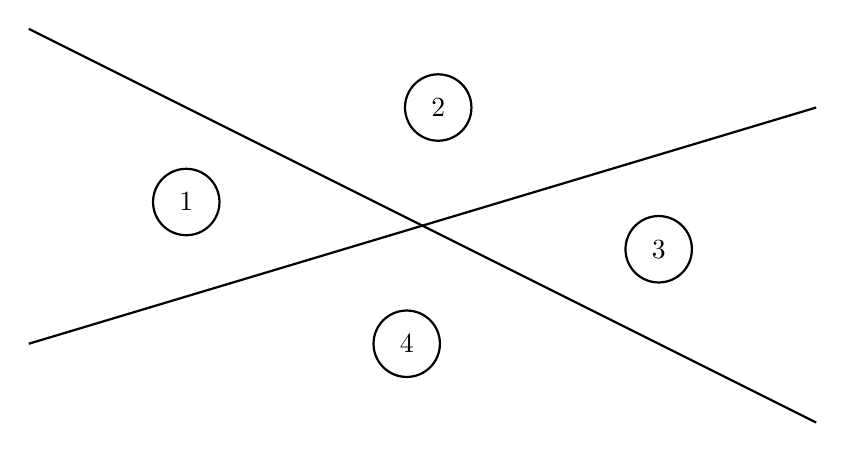
\begin{tikzpicture}[thick]
        \draw (-5,2.5) -- (5,-2.5);
        \draw (-5,-1.5) -- (5,1.5);
        \node[draw,circle,minimum size=24pt,inner sep=0,anchor=center] at (-0.2,-1.5) {$4$};
        \node[draw,circle,minimum size=24pt,inner sep=0,anchor=center] at (3,-0.3) {$3$};
        \node[draw,circle,minimum size=24pt,inner sep=0,anchor=center] at (-3,0.3) {$1$};
        \node[draw,circle,minimum size=24pt,inner sep=0,anchor=center] at (0.2,1.5) {$2$};
    \end{tikzpicture}
\end{center}

然而,这只是两条直线相交的\emph{特例}。如何证明\emph{任意}两条非平行直线\emph{总能}得到四个区域?也就是说,我们能否以某种方式结合直线数量 $n = 2$ 这一事实来描述这是\text{如何}发生的?思考一下!

下面是我们的方法。请注意,当我们添加第二条直线时,每个已经存在的区域都会被分成两部分,并且\emph{无论你如何绘制直线},只要确保两条直线不平行,结果都是这样。也就是说,如果我们用一条直线将平面分成两个区域,

\begin{center}
    \begin{tikzpicture}[thick]
        \draw (-5,2.5) -- (5,-2.5);
        \node[draw,circle,minimum size=24pt,inner sep=0,anchor=center] at (-3,0.3) {$1$};
        \node[draw,circle,minimum size=24pt,inner sep=0,anchor=center] at (0.2,1.5) {$2$};
    \end{tikzpicture}
\end{center}

然后添加一条新的直线会将每个现有区域分成两部分。这会向整个平面添加两个新的区域,总共四个区域:

\begin{center}
    \begin{tikzpicture}[thick]
        \draw (-5,2.5) -- (5,-2.5);
        \draw [color=red] (-5,-1.5) -- (0,0)  node[midway,below,sloped]{分割区域 1}
        -- (5,1.5) node[midway,above,sloped]{分割区域 2} ;
        \node[draw,circle,minimum size=24pt,inner sep=0,anchor=center,color=red] at (-0.2,-1.5) {$4$};
        \node[draw,circle,minimum size=24pt,inner sep=0,anchor=center,color=red] at (3,-0.3) {$3$};
        \node[draw,circle,minimum size=24pt,inner sep=0,anchor=center] at (-3,0.3) {$1$};
        \node[draw,circle,minimum size=24pt,inner sep=0,anchor=center] at (0.2,1.5) {$2$};
    \end{tikzpicture}
\end{center}

当 $n = 3$ 时呢?在这种情况下,我们需要考虑向具有两条直线和四个区域的图形中添加第三条直线。我们想要提出一个不依赖于线的特定排列的论证,因此我们最终唯一能用的事实是线之间互不平行,且任何交点仅位于两条线(而不是三条或更多)上。不过,就目前而言,查看特定的直线排列会有所启发,以便我们讨论相同的图形;我们可以利用对这个特定图形的观察来指导我们的一般论证。让我们从下方具有两条直线的图开始,向其中添加第三条直线,让第三条直线的交点都在初始交点``附近''或在图的范围内,这样我们就缩放图形了:

\begin{center}
    \begin{tikzpicture}[thick]
        \draw (-5,2.5) -- (5,-2.5);
        \draw (-5,-1.5) -- (5,1.5);
        \draw [color=red] (-5,1) -- (-1.8085,0.9043) node[midway,below,sloped]{\small 分割区域 1} 
        -- (2.5758,0.7727) node[midway,above,sloped]{\small 分割区域 2}
        -- (5,0.7) node[midway,below,sloped]{\small 分割区域 3};
        \node[draw,circle,minimum size=16pt,inner sep=0,anchor=center] at (-0.2,-1.5) {$4$};
        \node[draw,circle,minimum size=16pt,inner sep=0,anchor=center] at (3,-0.3) {$3$};
        \node[draw,circle,minimum size=16pt,inner sep=0,anchor=center] at (-3,-0.3) {$1$};
        \node[draw,circle,minimum size=16pt,inner sep=0,anchor=center] at (0.2,2) {$2$};
        \node[draw,circle,minimum size=16pt,inner sep=0,anchor=center,color=red] at (-4,1.45) {$5$};
        \node[draw,circle,minimum size=16pt,inner sep=0,anchor=center,color=red] at (0.1,0.45) {$6$};
        \node[draw,circle,minimum size=16pt,inner sep=0,anchor=center,color=red] at (4.61,1.05) {$7$};
    \end{tikzpicture}
\end{center}

很明显此时共有 $7$ 个区域。将第三条直线标绘为不同颜色,以便我们可以识别``新''区域出现的位置:一个区域(下方区域,区域 $4$)保持不变,但其他三个区域被一分为二,每次分割使区域计数加 $1$。如果我们以不同的方式绘制这条直线会怎样?

\begin{center}
    \begin{tikzpicture}[thick]
        \draw (-5,2.5) -- (5,-2.5);
        \draw (-5,-1.5) -- (5,1.5);
        \draw [color=red] (0,2.5) -- (-0.8333,0.4167) node[midway,right,sloped,rotate=-90]{\small 分割区域 2} 
        -- (-1.1364,-0.341) node[midway,left,sloped,rotate=-90]{\small 分割区域 1}
        -- (-2,-2.5) node[midway,right,sloped,rotate=-90]{\small 分割区域 4}; 
        \node[draw,circle,minimum size=16pt,inner sep=0,anchor=center] at (-0.2,-1) {$4$};
        \node[draw,circle,minimum size=16pt,inner sep=0,anchor=center] at (3,-0.3) {$3$};
        \node[draw,circle,minimum size=16pt,inner sep=0,anchor=center] at (-3,-0.3) {$1$};
        \node[draw,circle,minimum size=16pt,inner sep=0,anchor=center] at (1,2) {$2$};
        \node[draw,circle,minimum size=12pt,inner sep=0,anchor=center,color=red] at (-0.7,0.05) {$5$};
        \node[draw,circle,minimum size=16pt,inner sep=0,anchor=center,color=red] at (-1.5,1.8) {$6$};
        \node[draw,circle,minimum size=16pt,inner sep=0,anchor=center,color=red] at (-2.5,-1.4) {$7$};
    \end{tikzpicture}
\end{center}

类似的情况再次出现:其中一个区域保持不变,其余三个区域一分为二。(为何无其他区域?此问题值得深入思考。)尝试三条线的其他排列方式,并验证这种情况总会发生;此外,思考一下\emph{为什么}会出现这种情况,以及我们\emph{如何}解释这种情况一定会发生。不过,在给出一般性解释之前,我们再来看一下 $n=4$ 的情形。

当 $n = 4$ 时,我们从 $3$ 条直线和 $7$ 个区域的平面开始,添加第四条直线,该直线不与任何现有直线平行,并且不穿过任何现有交点。同样,我们想要提出一个与直线的特定排列无关的论证,但是查看下面的具体图形将有助于引导思路:

\begin{center}
    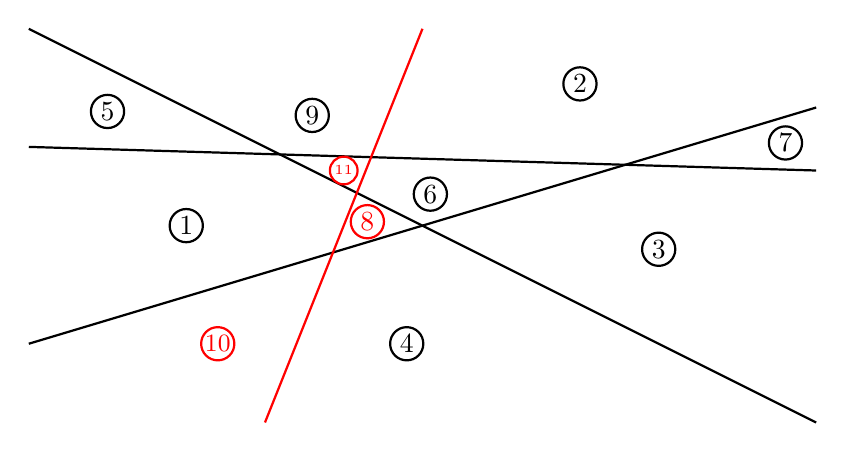
\begin{tikzpicture}[thick]
        \draw (-5,2.5) -- (5,-2.5);
        \draw (-5,-1.5) -- (5,1.5);
        \draw  (-5,1) -- (5,0.7);
        \draw [color=red] (0,2.5) -- (-2,-2.5);
        \node[draw,circle,minimum size=12pt,inner sep=0,anchor=center] at (-0.2,-1.5) {$4$};
        \node[draw,circle,minimum size=12pt,inner sep=0,anchor=center] at (3,-0.3) {$3$};
        \node[draw,circle,minimum size=12pt,inner sep=0,anchor=center] at (-3,0) {$1$};
        \node[draw,circle,minimum size=12pt,inner sep=0,anchor=center] at (2,1.8) {$2$};
        \node[draw,circle,minimum size=12pt,inner sep=0,anchor=center] at (-4,1.45) {$5$};
        \node[draw,circle,minimum size=12pt,inner sep=0,anchor=center] at (-1.4,1.4) {$9$};
        \node[draw,circle,minimum size=10pt,inner sep=0,anchor=center,color=red] at (-1,0.7) {\tiny $11$};
        \node[draw,circle,minimum size=12pt,inner sep=0,anchor=center] at (4.61,1.05) {$7$};
        \node[draw,circle,minimum size=12pt,inner sep=0,anchor=center,color=red] at (-0.7,0.05) {$8$};
        \node[draw,circle,minimum size=12pt,inner sep=0,anchor=center] at (0.1,0.4) {$6$};
        \node[draw,circle,minimum size=12pt,inner sep=0,anchor=center,color=red] at (-2.6,-1.5) {\small $10$};
    \end{tikzpicture}
\end{center}

请注意,三个原始区域保持不变(区域 $3$、区域 $5$ 和区域 $7$),而其他四个区域被一分为二。你注意到其中的规律了吗?对于每个已检验的 $n$,添加第 $n$ 条线会使 $n-1$ 个区域保持不变,其余区域则被一分为二。现在,让我们解释这一现象的原因。回忆一下,当绘制 $n$ 条直线时,我们的目标是确定区域的总数。为此,我们赋予该值一个名称以便引用:设 $R(n)$ 表示在平面上绘制 $n$ 条直线所创建的区域数,其中任意两条直线均不平行,且任意三条直线不共点。在上述示例中,我们考察了较小的 $n$ 值,并研究了添加新直线时的变化规律;也就是说,我们可以通过已知的 $R(n - 1)$ 推导 $R(n)$ 的值。现在,让我们将观察结果推广到适用于\emph{任意} $n$ 的情形。

假设已知 $R(n)$(为何可行?对于特定 $n$,我们是否确切知道 $R(n)$ 的值?它是什么?如何得知?)。考虑平面上满足题目条件的\emph{任意} $n$ 条直线图,这些直线将平面划分为 $R(n)$ 个区域。现在,添加第 $(n + 1)$ 条直线时会发生什么?关于这条直线如何改变图形,我们能确定哪些信息?关键约束如下:

\begin{enumerate}[label=(\alph*)]
    \item 新直线与现有的 $n$ 条直线均不平行;
    \item 新直线不经过任何现有交点。
\end{enumerate}

条件 (a) 表明新直线必与\emph{所有} $n$ 条已有直线相交(平行线无交点,非平行线必相交)。因此,新直线将产生 $n$ 个新交点。这些交点会与已有交点重合吗?不会!这正是条件 (b) 的作用。综上,只要满足题目要求,新直线上\emph{必定}存在 $n$ 个``特殊''点——即它与已有直线的交点。

接下来,我们利用这些特殊点识别新增区域。回顾之前的案例:标记新交点,并探究它们与新区域的关联。建议用圆点标记交点,并用 $\textbf{×}$ 标识新区域以增强可视性。下图展示了 $n = 4$ 的示例。你发现了什么?能否通过这些点推断添加第 $n$ 条直线后新增的区域数?思考一下,然后继续阅读。

\begin{center}
    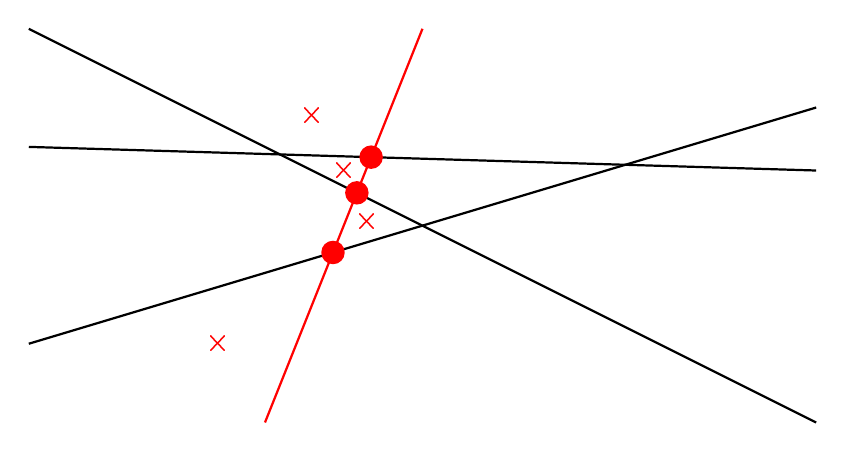
\begin{tikzpicture}[thick]
        \draw (-5,2.5) -- (5,-2.5);
        \draw (-5,-1.5) -- (5,1.5);
        \draw  (-5,1) -- (5,0.7);
        \draw [color=red] (0,2.5) -- (-2,-2.5);
        \node[minimum size=14pt,anchor=center,color=red,very thick] at (-1.4,1.4) {$\textbf{×}$};
        \node[minimum size=14pt,anchor=center,color=red,very thick] at (-1,0.7) {$\textbf{×}$};
        \node[minimum size=14pt,anchor=center,color=red,very thick] at (-0.7,0.05) {$\textbf{×}$};
        \node[minimum size=14pt,anchor=center,color=red,very thick] at (-2.6,-1.5) {$\textbf{×}$};
        \node[fill,circle,inner sep=3pt,color=red] at (-0.6522,0.8696) {};
        \node[fill,circle,inner sep=3pt,color=red] at (-0.8333,0.4167) {};
        \node[fill,circle,inner sep=3pt,color=red] at (-1.1364,-0.341) {};
    \end{tikzpicture}
\end{center}

没错!任意两个相邻新交点之间,都有一条\emph{线段}恰好将一个区域一分为二!接下来只需确定此类线段的数量即可。由于每条线段仅分割\emph{一个}已有区域,其数量即等于新增区域数。已知第 $(n + 1)$ 条直线产生 $n$ 个新交点。这些点在直线上如何排列?任意两个``连续'交点形成一条有限线段,而端点则延伸为无限射线(经端点无限延伸)。总计多少条线段?恰好 $n + 1$ 条(参考 $n = 3$ 的示意图:$3$ 个交点对应 $4$ 条线段,含两条无限射线)。因此,$n + 1$ 条线段分割出 $n + 1$ 个新区域,即:
\[R(n + 1) = R(n) + n + 1\]
出色的发现!通过分析示例和几何论证,我们成功揭示了递归关系:$R(n+1)$ 的值依赖于 $R(n)$。虽未完全解决问题,但已接近目标。接下来只需迭代展开 $R(n)$ 的表达式,直至已知的 $R(1) = 2$。过程如下:

\begin{center}
    \begin{tabular}{rcccccccccc}
        $R(n+1)$ & $=$ &          & &            &     &            &     & $\cancel{R(n-1)}$ & $+$ & $n+1$\\
                 & $=$ &          & &                   &     & $\cancel{R(n-1)}$ & $+$ & $n$ & $+$ & $n+1$\\
                 & $=$ &          & & $\cancel{R(n-2)}$ & $+$ & $(n-1)$           & $+$ & $n$ & $+$ & $n+1$\\
                 & $\vdots$ &     & &  &  &  &  &  &  & \\
                 & $=$ &          & & $\cancel{R(2)}+3$ & $+$ & $\dots$ & $+$ & $n$ & $+$ & $n+1$ \\
                 & $=$ & $R(1)+2$ & $+$ & $3$               & $+$ & $\dots$ & $+$ & $n$ & $+$ & $n+1$ \\
    \end{tabular}
\end{center}

由 $R(1) = 2$ 可得:
\[R(n + 1) = 2 + \left(2 + 3 + \dots + n + (n + 1)\right) = 2 + \left(\sum_{k=1}^{n+1}k\right)-1 = 1+\sum_{k=1}^{n+1}k\]
而这正是我们之前研究过的求和公式!(注意括号内求和缺首项 $k=1$,故需减去 $1$)。回忆 $\sum_{k=1}^{n} k = \frac{n(n+1)}{2}$,为了表示上面等式中的求和,我们只需将 $n$ 替换为 $n + 1$ 即可。因此,
\[R(n + 1) = 1+\frac{(n+1)(n+2)}{2}\]
最后,为得到 $R(n)$ 的显式表达式,将 $n+1$ 替换为 $n$(对 $n$ 的取值有什么要求?):
\[R(n + 1) = 1+\frac{n(n+1)}{2}\]
至此,我们获得了原问题的答案!此过程运用了\emph{归纳}技术:通过建立 $R(n + 1)$ 对 $R(n)$ 的依赖关系,反向迭代至\emph{已知}值 $R(1)$。

需要强调的是,本节推导旨在引导直觉而非提供\emph{严格证明}。省略号(``$\dots$'')并非严谨的数学归纳表述。此外,我们的方法是从 $n - 1$ 条直线出发\emph{逐步构建} $n$ 条直线的情形——这是否合理?为何能推广到 $n$ 条直线的\emph{任意}图?所有此类图是否均来自少一条线的子图?

接下来的两章将引入严格工具以形式化上述方法,并建立数学归纳的严谨框架。当前阶段,我们仅提供归纳法的启发式定义,并继续探索依赖归纳的有趣问题。重点在于练习识别归纳结构、运用其解决问题等技能,这对未来学习至关重要(暂无需深入数学细节!)。


% !TeX root = ../../../book.tex
\subsection{习题}

\subsubsection*{温故知新}

以口头或书面的形式简要回答以下问题。这些问题全都基于你刚刚阅读的内容,所以如果忘记了具体的定义、概念或示例,可以回去重读相关部分。确保在继续学习之前能够自信地回答这些问题,这将有助于你的理解和记忆!

\begin{enumerate}[label=(\arabic*)]
    \item 归纳过程有哪些特征?
    \item 我们如何证明 $\sum_{k=1}^{n}k = \frac{n(n+1)}{2}$ 是正确的?我们的方法是如何归纳的?(如果你不记得了,请重读第 \ref{sec:section1.4.2} 节!)
    \item 为什么我们可以把上一个问题中提到的求和公式,用 $n+1$ ``替换'' $n$,并且知道它仍然成立?我们也可以将 $n$ 替换为 $n - 1$ 吗?
    \item 通过代数步骤获得前 $n$ 个自然数平方和的最终表达式;也就是说,验证
    \[\frac{1}{3}(n+1)^3-\frac{1}{3}(n+1)-\frac{n(n+1)}{2} = \frac{1}{6}n(n+1)(2n+1)\]
    \item 试着回忆一下向平面中添加第 $(n+1)$ 条直线正好会创建 $n+1$ 个新区域的论点。你能为朋友证明这个论点并说服他/她它是有效的吗?
    \item 求前 $n$ 个自然数的平方和,为什么不能把前 $n$ 个自然数之和的公式平方呢?为什么这是错误的?
\end{enumerate}

\subsubsection*{小试牛刀}

尝试回答以下问题。这些题目要求你实际动笔写下答案,或(对朋友/同学)口头陈述答案。目的是帮助你练习使用新的概念、定义和符号。题目都比较简单,确保能够解决这些问题将对你大有帮助!

\begin{enumerate}[label=(\arabic*)]
    \item 在平面中画 $5$ 条直线(满足原题的两个条件)并验证是否有 $16$ 个区域。你还能验证 $6$ 条线产生 $22$ 个区域吗?
    \item 给出序列 $1, 2, 3, 4, \dots , 100$ 的另一种解释,而不仅仅是从 $1$ 到 $100$ 的所有自然数。(回想一下我们给出的例子:$1$ 到 $100$ 之间所有英文拼写中不含字母"i"的数字。)
    \item 提出一个将 $(n + 1)^4$ 与 $n^4$ 联系起来的代数表达式,就像我们对立方所做的那样。\\ 
    (\textbf{挑战题:}你能为刚刚推导出的表达式给出\emph{几何}解释吗?)
    \item \textbf{挑战题:}让我们将``平面上的线''这题提升一个维度!考虑三维空间中有 $n$ 个平面。会创建多少个区域?假设没有两个平面平行,并且没有三个或以上平面相交于一条直线。(想想这两个条件如何直接类比于``线''那题的给定条件。)
\end{enumerate}

\newpage
% !TeX root = ../../../book.tex
\section{定义归纳}

为了将数学归纳法定义为证明技术,我们想强调,上一节中的例子使用了问题结构的某些直观概念来给出问题的``解'',我们在\emph{解}上加了引号,表明我们还没有正式证明它。从这个意义上讲,我们提出以下问题:如果\emph{给定}我们前面推导的公式并要求验证它怎么办?如果我们没有通过任何直观的步骤来推导公式,只是有人告诉我们它是正确的怎么办?我们如何验证他们的说法?之所以问这个问题,是因为我们现在确实面临着这种情况,除非告诉我们公式的人采用与我们相同的直觉论证。

假如一个持怀疑态度的朋友说:``嘿,我听说过一个计算前 $n$ 个自然数平方和的公式。有人告诉我,它们加起来等于 $\frac{1}{6}n(n+1)(2n+1)$。我验证了前两个自然数,全都正确,所以它一定是正确的。应该传播出去!'' 作为一个理性思考者,同时也是好朋友的身份,你点点头说:``我确实听说了,但让我们确保这个公式对每个数字都是正确的。'' 你将如何进行?你的朋友说的没错,前几个值确实``完美匹配'':

\begin{align*}
    1^2 &= \enspace 1 = \frac{1}{6}(1)(2)(3) \\
    1^2 + 2^2 &= \enspace 5 = \frac{1}{6}(2)(3)(5) \\
    1^2 + 2^2 + 3^2 &= 14 = \frac{1}{6}(3)(4)(7) \\
    1^2 + 2^2 + 3^2 + 4^2 &= 30 = \frac{1}{6}(4)(5)(9)
\end{align*}
如果我们愿意的话,我们甚至可以手动检验 $n$ 的更大的值:
\[1^2 + 2^2 + 3^2 + 4^2 + 5^2 + 6^2 + 7^2 + 8^2 + 9^2 + 10^2 = 385 = \frac{1}{6}(10)(11)(21)\]
但请记住,该公式声称对于\emph{任意} $n$ 值都有效。手动检验每个结果将花费大量时间,因为自然数有\emph{无穷}多个。无论我们检验多少个独立的 $n$ 值,总会有更大的值,我们怎么\emph{知道}公式对于某些大值不会失效?从数学和时间上来讲,我们需要一个更加\emph{有效}的方法,以某种方式只需几步即可验证所有 $n$ 值。我们先在心里埋下一颗种子(这是即将推出的数学归纳法的严格版本),在这里我们将从广义上解释该过程是如何工作的。

% !TeX root = ../../../book.tex
\subsection{多米诺骨牌类比}

假设我们有一副特殊的多米诺骨牌,它包含无穷多张骨牌!每张骨牌可以书写任意内容,而非标准的点数。这些骨牌沿无限延伸的桌面排列成无限长的一行。从侧面观察时,每张骨牌下方标有位置标签:

\begin{center}
    \begin{tikzpicture}
        \foreach \x in {1,...,5}
        {
            \pic [fill=white] at (\x, 0, 0) {annotated cuboid={width=3, height=30, depth=10}};
            \node[below] at (\x, -3){\tiny $n=\x$};
        }
        \node[anchor=center] at (6.5, -1.5){\LARGE $\dots \cdot$};
        % \pic [very thick,densely dashed,draw=blue] at (5,0) {annotated cuboid={width=30, height=5, depth=10, opacity=0.2}};
    \end{tikzpicture}
\end{center}

对于这个特定的例子,我们需要验证公式
\[\sum_{k=1}^{n}k^2 = \frac{1}{6}n(n+1)(2n+1)\]
为此,设想每张多米诺骨牌记载一个特定``事实''。具体来说,我们可以想象第一张多米诺骨牌上写有表达式
\[\sum_{k=1}^{1}k^2 = \frac{1}{6}(1)(1)(3)\]
第二张多米诺骨牌上写有表达式
\[\sum_{k=1}^{2}k^2 = \frac{1}{6}(2)(3)(5)\]
推而广之,第 $n$ 张骨牌写有如下``事实'':
\[\sum_{k=1}^{n}k^2 = \frac{1}{6}n(n+1)(2n+1)\]
由于多米诺骨牌具有连锁倾倒的特性,我们约定骨牌倒下即表示其记载的``事实''是\emph{真实命题}。由此将多米诺骨牌的物理解释与公式有效性的数学解释联系起来。

我们已手动验证 $n=1$ 的情形:$1^2=\frac{1}{6}(1)(2)(3)$,故第一张骨牌记载的命题为真,必将倒下。同理验证 $n=2$ 后,第二张骨牌也会倒下:

\begin{center}
    \begin{tikzpicture}
        \foreach \x in {1,2}
        {
            \pic [fill=white, rotate=-30, anchor=south] at (\x, -0.15, 0) {annotated cuboid={width=3, height=32, depth=10}};
            \node[below] at (\x-1.5, -3){\tiny $n=\x$};
        }
        \foreach \x in {3,4,5}
        {
            \pic [fill=white] at (\x, 0, 0) {annotated cuboid={width=3, height=30, depth=10}};
            \node[below] at (\x, -3){\tiny $n=\x$};
        }
        \node[anchor=center] at (6.5, -1.5){\LARGE $\dots \cdot$};
        % \pic [very thick,densely dashed,draw=blue] at (5,0) {annotated cuboid={width=30, height=5, depth=10, opacity=0.2}};
    \end{tikzpicture}
\end{center}
然而,若继续逐个检验,又会陷入原先的困境——我们不可能验证\emph{每张}骨牌。真正的需求是捕捉多米诺效应的精髓:一张骨牌倒下将触发下一张倒下。这要求我们建立相邻骨牌所载``事实''的数学关联。

让我们看看前两张多米诺骨牌的情况。既然知道骨牌 $1$ 倒下,我们能否在不重写所有求和项的情况下确保骨牌 $2$ 倒下?两块骨牌上的陈述有何关联?每个陈述都是自然数的平方和,且第二张骨牌的陈述正好多出一项。因此,利用骨牌 $1$ 上已知的\emph{真实陈述},可以\emph{验证}骨牌 $2$ 上陈述的真实性:
\[\sum_{k=1}^{2}k^2 = 1^2+2^2=1+2^2=5=\frac{1}{6}(2)(3)(5)\]
尽管节省的唯一``工作''只是免于计算 $1^2=1$,但让我们在更大数字上应用此过程以凸显其优势。\emph{假设}骨牌 $10$ 已经倒下(其求和的完整验证已在前文给出),这意味着我们\emph{知道}
\[\sum_{k=1}^{10}k^2 =\frac{1}{6}(10)(11)(21)=285\]
是一个\emph{真实陈述}。利用它来验证骨牌 $11$ 的陈述:
\[\sum_{k=1}^{11}k^2 =\frac{1}{6}(11)(12)(23)\]
骨牌 $11$ 上的求和公式有 $11$ 项,前 $10$ 项正是骨牌 $10$ 上的求和!因此只需分离第 $11$ 项并代入已知结果:
\begin{align*}
    \sum_{k=1}^{11}k^2 &= (1^2+2^2+\dots+10^2)+11^2\\
    &=\sum_{k=1}^{10}k^2+11^2\\
    &=385+121\\
    &=506\\
    &=\frac{1}{6}3036=\frac{1}{6}(11)(12)(23)
\end{align*}
节省的工作量显而易见!既然已知前 $10$ 项之和,何必重新计算?

现在设想对\emph{所有} $n$ 值\emph{同时}实施此过程!若能证明每当骨牌 $n$ 倒下,骨牌 $(n + 1)$ \emph{必然}倒下,这意味着什么?回顾无穷骨牌序列:已知骨牌 $1$ 因手动检验而倒下,加之``骨牌 $n$ 撞倒骨牌 $(n + 1)$''的普适性验证,可推得骨牌 $1$ 撞倒骨牌 $2$,骨牌 $2$ 撞倒骨牌 $3$,骨牌 $3$ 撞倒骨牌 $4$,…… 如此传递下去,整列骨牌终将全部倒下!本质上,整个过程可归结为\emph{两步}:

\begin{enumerate}[label=(\arabic*)]
    \item 确保第一张骨牌倒下;
    \item 确保每张骨牌都能撞倒下一张骨牌。
\end{enumerate}
仅凭这两步,便能\emph{保证}所有骨牌倒下,从而\emph{证明}每个公式对\emph{任意}自然数 $n$ 成立。

我们已经完成步骤 (a),现在需要完成步骤 (b)。此前已针对特定案例(骨牌 $1$ 撞倒骨牌 $2$、骨牌 $10$ 撞倒骨牌 $11$)执行了此操作,现在将其推广到任意 $n$ 值。我们\emph{假设}:对于某个\emph{特定}但\emph{任意}的 $n$,多米诺骨牌 $n$ 会倒下,这意味着方程
\[\sum_{k=1}^{n}k^2=\frac{1}{6}n(n+1)(2n+1)\]
为\emph{真实陈述}。现在需将其关联到骨牌 $(n+1)$ 的陈述,并应用上述等式信息。将 $n+1$ 项的和拆分为 $n$ 项和与末项:
\[\sum_{k=1}^{n+1}k^2 = (1^2+2^2+\dots+n^2+(n+1)^2)=\sum_{k=1}^{n}k^2+(n+1)^2\]
根据骨牌 $n$ 倒下的假设(即其命题为真),可得
\[\sum_{k=1}^{n+1}k^2 = \frac{1}{6}n(n+1)(2n+1)+(n+1)^2\]
这与骨牌 $(n+1)$ 的命题是否一致?骨牌 $(n+1)$ 的``事实''与骨牌 $n$ 类似,只是将``$n$''替换为``$n + 1$'':
\[\sum_{k=1}^{n+1}k^2 = \frac{1}{6}\big(n+1\big)\big((n+1)+1\big)\big((2(n+1)+1)\big)=\frac{1}{6}(n+1)(n+1)(2n+3)\]
目前还不清楚我们推导出的表达式是否实际上等于上面的式子。我们可以尝试化简该表达式,并将其分解为与上面表达式``类似''的新表达式,但展开两个表达式并比较所有项可能会更容易。(这基于这样的一般思想:展开因式分解后的多项式比进行因式分解要容易得多。)对于第一个表达式,我们有
\begin{align*}
    \frac{1}{6}n(n + 1)(2n + 1) + (n + 1)^2 &=\frac{1}{6}n(2n^2 + 3n + 1) + (n^2 + 2n + 1)\\
    &= \frac{1}{3}n^3 + \frac{1}{2}n^2 + \frac{1}{6}n + n^2 + 2n + 1 \\
    &= \frac{1}{3}n^3 + \frac{3}{2}n^2 + \frac{13}{6}n + 1
\end{align*}
对于第二个表达式,我们有
\begin{align*}
    \frac{1}{6}(n+1)(n + 2)(2n + 3) &=\frac{1}{6}(n+1)(2n^2 + 7n+6)\\
    &= \frac{1}{6}\big[(2n^3 + 7n^2 + 6n) + (2n^2 + 7n + 6)\big] \\
    &= \frac{1}{3}n^3 + \frac{3}{2}n^2 + \frac{13}{6}n + 1
\end{align*}
可见两式相等!此外,请注意,这比尝试整理其中一个表达式并将其``变形''为另一个表达式要容易得多。我们通过展开两式并最终得到相同的表达来证明它们是相同的。现在,让我们回顾并总结我们所取得的成果:
\begin{enumerate}
    \item 我们将证明公式
    \[\sum_{k=1}^{n+1}k^2 = \frac{1}{6}n(n+1)(2n+1)+(n+1)^2\]
    对于\emph{所有} $n$ 值成立类比为推倒无穷多的多米诺骨牌。
    \item 通过手工计算验证骨牌 $1$ 的命题成立,骨牌 $1$ 倒下;
    \item \emph{假设}骨牌 $n$ 的命题为真,由骨牌 $n$ 命题成立推出骨牌 $(n+1)$ 命题成立,从而证明骨牌 $n$ 会撞倒骨牌 $(n+1)$。
    \item 由此保证所有骨牌都会倒下,因此公式对\emph{所有} $n$ 都成立。
\end{enumerate}
此方法是否严谨?是否已\emph{严格证明}公式对所有自然数 $n$ 都成立?若存在 $n$ 使得公式失效,这对多米诺骨牌体系意味着什么?

请记住,这里的多米诺骨牌类比只是理解归纳法工作原理的一个直观指引,并非建立在严格的数学基础之上。建立严格的数学基础将是接下来几章的目标。现在,让我们回顾本章讨论的另一个例子:直线划分平面区域。同样,在推导公式 $R(n)$ 时使用省略号显得繁琐,我们希望避免这种做法。让我们尝试将多米诺骨牌类比应用于此问题。

设想我们定义 $R(n)$ 为 $n$ 条直线在平面上划分出的不同区域的数量,这些直线满足互不平行且任意三条(或更多)直线不共点。进一步设想,我们在代表第 $n$ 步的骨牌上写下``$R(n) = 1 + \frac{n(n+1)}{2}$''这一``事实''。能否按照与之前相同的逻辑来验证所有骨牌都会倒下?

首先,需要验证骨牌 $1$ 是否会倒下。这等同于验证命题``$R(1) = 1+\frac{1(2)}{2} = 1+1 = 2$''是否成立。这显然成立,正如我们之前验证过的:一条直线将平面划分为两个区域。其次,需要证明对于\emph{任意} $n$,第 $n$ 块骨牌倒下必定导致第 $(n + 1)$ 块骨牌倒下。也就是说,我们\emph{假设}``$R(n) = 1 + \frac{n(n+1)}{2}$''对某个特定的 $n$ 成立,然后\emph{证明}``$R(n + 1) = 1 + \frac{(n+1)(n +2)}{2}$''也必然成立。如何证明?沿用之前的思路,建立 $R(n + 1)$ 与 $R(n)$ 的关系。向\emph{任意}满足条件的 $n$ 条直线的图形中添加一条新直线,通过几何分析,我们得到关系式 $R(n+1) = R(n) + n + 1$。利用此关系以及第 $n$ 块骨牌倒下的假设,可得:
\[R(n + 1) = R(n) + n + 1 = 1 +\frac{n(n+1)}{2}+ n + 1\]
这个结果是否与骨牌 $(n + 1)$ 上的表达式一致?通过化简比较即可验证:
\[1 +\frac{n(n+1)}{2}+ n + 1=2+n+\frac{n^2+n}{2} = \frac{1}{2}n^2+\frac{3}{2}n+2\]
以及
\[1 + \frac{(n+1)(n +2)}{2} = 1+\frac{n^2+3n+2}{2} =  \frac{1}{2}n^2+\frac{3}{2}n+2\]
结果完全相同!因此,我们证明了对于\emph{任意} $n$,骨牌 $n$ 倒下\emph{必然}导致骨牌 $(n+1)$ 倒下。

思考一下,使用这种``多米诺骨牌技术''进行的证明,与我们之前为推导该公式所采用的方法有何不同?我们在本节中是否使用了省略号?为何这种证明方式更优?我们是否曾用多米诺骨牌归纳技术来推导公式本身?


% !TeX root = ../../../book.tex
\subsection{其他类比}

多米诺骨牌类比非常流行,但它并不是归纳法工作方式的唯一描述。根据你的阅读内容或交谈对象,可能会学到不同的类比,或其他类型的描述。这里,我们将描述以前听说过的两个。思考这些类比本质上的等价性,这将有助于巩固你对归纳法的理解(至少就我们所开发的而言)。

\subsubsection*{神奇的数学猴子 Mojo}

想象一个无穷天梯,直矗云霄。梯子有无数级,按 $1, 2, 3$ 的顺序依次编号。我们的朋友 Mojo 恰好站在梯子旁。他是一只聪明的猴子,对数学很感兴趣,但也有点神奇,因为他真的可以爬上这个无穷天梯!

如果 Mojo 到达了阶梯上的某一级,则意味着与该数字对应的事实为真。我们怎样才能确保他爬完整个梯子?单独检查每个阶梯的效率很低。想象一下:我们必须站在地面上确保他到达第 $1$ 级,然后我们必须稍微抬起头来确保他到达了第 $2$ 级,然后是第 $3$ 级,依此类推……相反,我们在 Mojo 开始攀爬之前确认了两个细节。他要开始攀爬了吗?也就是说,他会爬上第 $1$ 级吗?如果是这样,那就太好了!另外,阶梯之间的距离是否足够近,以便无论他在哪里,\emph{总能}到达下一个阶梯?如果是这样,那就更棒了!这些与我们在多米诺骨牌类比中建立的条件完全相同。为了确保 Mojo 到达\emph{每个}阶梯,我们只需要知道他到达了第 $1$ 个阶梯,并且他总是可以到达下一个阶梯。

\subsubsection*{归纳鸭 Doug}

再来认识一下 Doug。他是一只鸭子。他喜欢面包,所以他会去每个人的院子里寻找更多的面包。这些院子都沿数学镇的归纳街而建,房子的编号是 $1, 2, 3, \dots$ 以此类推。

Doug 从 $1$ 号院子开始寻找面包。没有找到任何东西,所以他依旧很饿。还能去哪里找?隔壁还有 $2$ 号院子!Doug 朝那边走去,肚子咕咕叫。他在那里也没找到面包,所以他必须继续寻找。此时他已经知道 $1$ 号院子没有面包,所以唯一去向就是隔壁的 $3$ 号院子。我想你已经明白事情的发展方向了…… 

如果我们跟踪 Doug 的进展,我们可能想知道他最终是否到达了每一个院子。假设我们已经提前知道\emph{没人}有面包。这意味着,每当 Doug 在某个院子里时,他一定会去隔壁院子,继续寻找食物。这意味着他一定会挨家挨户地去寻找!也就是说,无论我们住在哪栋房子里,无论我们门前的数字多大,在某个时点我们一定会看到 Doug 在我们的后院闲逛。(不幸的是,他会一直饿着肚子!可怜的 Doug。)


% !TeX root = ../../../book.tex
\subsection{总结}

回顾前两个示例的工作及我们的类比,可以发现每个问题都具有特定的\emph{结构}:某个``事实''依赖于``前一个事实''。对于立方数,我们找到了用 $n^3$ 表示 $(n + 1)^3$ 的方法;对于平面分割问题,我们刻画了向 $n$ 条直线的图形添加新直线时新增的区域个数。基于这些观察,我们反复应用已知关系,直至抵达一个可验证的``基础事实''——通常对应较小的 $n$ 值(两例中均为 $n = 1$)。这一过程使我们能够推导出适用于\emph{任意} $n$ 的通用公式或表达式。

尽管这项工作对公式推导至关重要且富有启发性,但它本身\emph{不足以证明}公式的有效性。在进行上述工作时,我们发现了归纳过程的存在,并利用其结构推导了相关表达式。这实际上有两个好处:不仅发现了待证公式,还让我们意识到采用\emph{数学归纳法}进行严格证明的可行性。

实际的``归纳证明''包含两个核心步骤:首先,验证公式在某个``起始值''成立;其次,\emph{假设}公式对某个特定 $n$ 成立,并以此证明其对 $n + 1$ 必然成立。完成这两步后,我们即可断言``所有多米诺骨牌都会倒下''——公式对所有相关 $n$ 值都成立。

\subsubsection*{一个问题:梯子的``尽头''是什么?}

你可能仍存疑虑,我们尝试在此预测你的担忧。(之所以提及这一点,是因为这是一个常见疑问。若你\emph{未曾}考虑这一点,请试着想象其来源。)你或许会说:``等等,现在我明白 Mojo 如何攀登天梯了,但他如何真正\emph{抵达顶端}呢?这是个无穷阶梯,对吗?那他永远无法到达终点……不是吗?''

某种意义上,你是对的。既然这个神奇阶梯将\emph{永远}延伸,它便没有真正的终点,Mojo 永无法抵达``顶端''。然而,这并非关键;我们不在意任何``\emph{顶端}''(不仅仅是因为\emph{不存在}顶端),只需确认 Mojo 能踏足\emph{每一个}台阶。他不必凌驾所有台阶立于顶端俯视来路——那不是目的!知道 Mojo 实际上到达了\emph{每一个可能的}阶梯。他不必超越所有人,站在梯子的顶端,俯视自己的来路。那不是目标!

不妨这样思考:假设你对某个待证事实抱有浓厚兴趣,例如
\[\text{事实\ } \#18,458,789,572,311,000,574,003 \text{\ (具体数值无关紧要)}\]
它对应遥不可及的台阶,而你只关心 Mojo 能否抵达。他会到达吗?他当然会!这或许需要漫长的时光(多少步呢?),但这在猴子与梯子的神奇世界,谁又在乎时间呢?你知道他终将抵达,这就够了。试想每个事实在神奇世界里都有专属关注者,每位关注着都将因 Mojo 踏足其关切之阶而欣喜。无人在意他能否登顶——那并非焦点。与此同时,在现实世界中,我们因\emph{所有}关注者终将如愿而欣慰。无限攀登的过程被简化为两步:仅凭此两步,我们便确信阶梯的\emph{每一级}皆可达,每个编号的事实皆成立。

亦可类比多米诺骨牌:我们是否在意骨牌链存在``终点'',最终撞上墙壁?当然不。骨牌链将永续延伸,每张牌终会倒下,时间长短无关紧要。同理,我们知晓 Doug 终将抵达\emph{所有}院子——何时抵达\emph{某个}院子无关紧要,唯有抵达\emph{全部}院子方为关键。


% !TeX root = ../../../book.tex
\subsection{习题}\label{sec:section2.3.4}

\subsubsection*{温故知新}

以口头或书面的形式简要回答以下问题。这些问题全都基于你刚刚阅读的内容,如果忘记了具体定义、概念或示例,可以回顾相关内容。确保在继续学习之前能够自信地作答这些问题,这将有助于你的理解和记忆!

\begin{enumerate}[label=(\arabic*)]
    \item 多米诺骨牌、Mojo 和 Doug 的类比为何等价?能否定义一个``函数''来描述它们之间的关系,实现类比间的相互转换?
    \item 找一位未接触过数学归纳法的朋友,尝试向他解释这一概念。你是否在解释中使用了上述类比?这些类比是否有帮助?
    \item 为什么我们对立方体的研究不足以证明求和公式?为何仍需完成后续推导?
    \item 思考多米诺骨牌的类比:若骨牌无限延伸是否会导致某些骨牌永不倒下?尝试用类比解释这一现象的含义。
\end{enumerate}

\subsubsection*{小试牛刀}

尝试解答以下问题。这些题目需动笔书写或口头阐述答案,旨在帮助你熟练运用新概念、定义及符号。题目难度适中,确保掌握它们将大有裨益!

\begin{enumerate}[label=(\arabic*)]
    \item 用数学归纳法证明公式:
    \[\sum_{k=1}^{n}k = \frac{n(n+1)}{2}\]
    \item 用数学归纳法证明公式:
    \[\sum_{k=1}^{n}2k-1 = n^2\]
    \item 用数学归纳法证明公式:
    \[\sum_{k=1}^{n}k^3 = \Bigg(\frac{n(n+1)}{2}\Bigg)^2\]
    \item 设存在一系列由自然数索引的命题,用``$P(n)$''表示第 $n$ 个命题。
    \begin{enumerate}[label=(\alph*)]
        \item 若要证明对所有自然数 $n$,\emph{每个} $P(n)$ 均成立,应该如何操作?
        \item 若只需证明当 $n$ 为\emph{偶数}时 $P(n)$ 成立,应该如何处理?能否通过修改某个类比来描述此方法?
        \item 若只需证明当 $n \geq 4$ 时 $P(n)$ 成立,又该如何处理?能否通过修改某个类比来描述此方法?
    \end{enumerate}
\end{enumerate}


\newpage
% !TeX root = ../../../book.tex
\section{另外两个(不同的)例子} \label{sec:section2.4}

本节有两个主要目的。首先,我们旨在避免读者产生归纳法仅适用于证明\emph{数值公式}(如涉及数字或多项式)的误解。归纳法的应用远比这广泛得多!特别是接下来的例子将证明:某些抽象性质对于给定情境中的任意``规模''均成立。我们会看到这仍属于``归纳''的范畴,同时也能观察到其与先前例子的区别。此外,这些例子还揭示了一个重要现象:有时推动多米诺骨牌需要掌握``更多信息''。在之前的案例中,仅需确认骨牌 $n$ 倒下,即可\emph{确保}骨牌 $n + 1$ 随之倒下。但在本节的示例中,我们可能需要了解前几个骨牌的状态。通过这两个例子,我们将总结其与前述多米诺骨牌模型的差异,并预览适用于此类情况的、更通用的归纳技术定义。

% !TeX root = ../../../book.tex
\subsection{多米诺与密铺} \label{sec:section2.4.1}

下面的示例比前两个示例稍微复杂一些。我们最终仍将证明某个数值公式,但问题显然比仅仅操纵代数表达式更加直观。此外,我们会在开始步骤中注意到一个有趣的``问题'',即我们必须解决几个``小案例'',然后才能推广我们的方法。这将是我们首次考虑如何泛化归纳技术使其适应其他情况。

我们要回答的问题可以表述如下:

\begin{quote}
    给定一个 $2 \times n$ 的正方形棋盘,有多少种不同的方式可以用多米诺骨牌平铺该棋盘?平铺必须让每个正方形都被一块——且只有一块——多米诺骨牌覆盖。
\end{quote}
例如,以下是正确的密铺

\begin{center}
    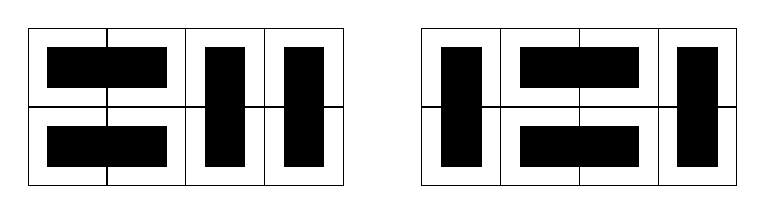
\begin{tikzpicture}[x=1.0cm, y=1.0cm]
        \foreach \y in {0,1} {
            \foreach \x in {0,...,3} {
                \draw (0+\x ,0+\y) rectangle ++ (1,1);
            }
        }

        \draw[fill, black] (0.25 ,0.25) rectangle ++ (1.5,0.5);
        \draw[fill, black] (0.25 ,1.25) rectangle ++ (1.5,0.5);
        \draw[fill, black] (2.25 ,0.25) rectangle ++ (0.5,1.5);
        \draw[fill, black] (3.25 ,0.25) rectangle ++ (0.5,1.5);

        \foreach \y in {0,1} {
            \foreach \x in {0,...,3} {
                \draw (5+\x ,0+\y) rectangle ++ (1,1);
            }
        }

        \draw[fill, black] (5+1.25 ,0.25) rectangle ++ (1.5,0.5);
        \draw[fill, black] (5+1.25 ,1.25) rectangle ++ (1.5,0.5);
        \draw[fill, black] (5+0.25 ,0.25) rectangle ++ (0.5,1.5);
        \draw[fill, black] (5+3.25 ,0.25) rectangle ++ (0.5,1.5);
    \end{tikzpicture}
\end{center}
而以下\emph{不}是正确的密铺

\begin{center}
    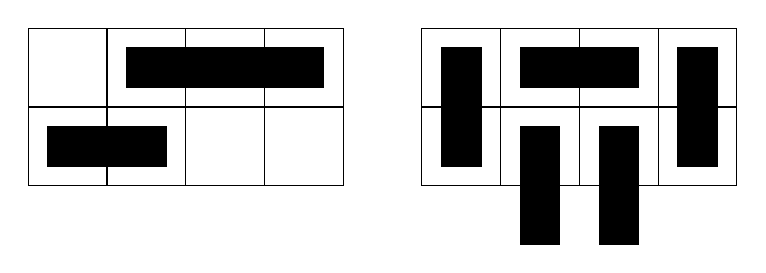
\begin{tikzpicture}[x=1.0cm, y=1.0cm]
        \foreach \y in {0,1} {
            \foreach \x in {0,...,3} {
                \draw (0+\x ,0+\y) rectangle ++ (1,1);
            }
        }

        \draw[fill, black] (0.25 ,0.25) rectangle ++ (1.5,0.5);
        \draw[fill, black] (1.25 ,1.25) rectangle ++ (1.5,0.5);
        \draw[fill, black] (2.25 ,1.25) rectangle ++ (1.5,0.5);

        \foreach \y in {0,1} {
            \foreach \x in {0,...,3} {
                \draw (5+\x ,0+\y) rectangle ++ (1,1);
            }
        }

        \draw[fill, black] (5+1.25 ,1.25) rectangle ++ (1.5,0.5);
        \draw[fill, black] (5+1.25 ,-0.75) rectangle ++ (0.5,1.5);
        \draw[fill, black] (5+2.25 ,-0.75) rectangle ++ (0.5,1.5);
        \draw[fill, black] (5+0.25 ,0.25) rectangle ++ (0.5,1.5);
        \draw[fill, black] (5+3.25 ,0.25) rectangle ++ (0.5,1.5);
    \end{tikzpicture}
\end{center}

和以前一样,让我们查看前几种情况(其中 $n = 1, 2, 3$ 等),看看我们是否能发现任何模式。在继续阅读之前,尝试自己解决该问题!

当 $n = 1$ 时,我们有一个与多米诺骨牌形状完全相同的棋盘,因此肯定只有一种方法可以密铺。让我们使用符号 $T(n)$ 来表示 $2 \times n$ 棋盘上的密铺数量。因此,$T(1) = 1$。

\begin{center}
    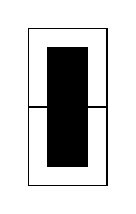
\begin{tikzpicture}[x=1.0cm, y=1.0cm]
        \draw (0,0) rectangle ++ (1,1);
        \draw (0,1) rectangle ++ (1,1);
        \draw[fill, black] (0.25 ,0.25) rectangle ++ (0.5,1.5);
    \end{tikzpicture}
\end{center}
当 $n = 2$ 时,我们有一个 $2 \times 2$ 棋盘。由于棋盘的方向很重要,因此我们有以下两种不同的密铺。因此,$T(2) = 2$。

\begin{center}
    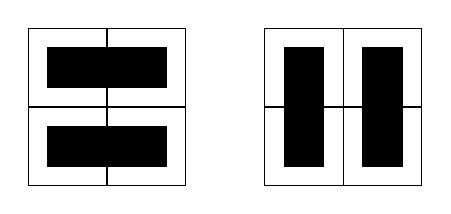
\begin{tikzpicture}[x=1.0cm, y=1.0cm]
        \foreach \y in {0,1} {
            \foreach \x in {0,1} {
                \draw (0+\x ,0+\y) rectangle ++ (1,1);
            }
        }

        \draw[fill, black] (0.25 ,0.25) rectangle ++ (1.5,0.5);
        \draw[fill, black] (0.25 ,1.25) rectangle ++ (1.5,0.5);

        \foreach \y in {0,1} {
            \foreach \x in {0,1} {
                \draw (3+\x ,0+\y) rectangle ++ (1,1);
            }
        }

        \draw[fill, black] (3+0.25 ,0.25) rectangle ++ (0.5,1.5);
        \draw[fill, black] (3+1.25 ,0.25) rectangle ++ (0.5,1.5);
    \end{tikzpicture}
\end{center}
当 $n = 3$ 时呢?同样地,我们可以手动枚举这些密铺,并确保没有遗漏任何一个。我们看到 $T(3) = 3$。

\begin{center}
    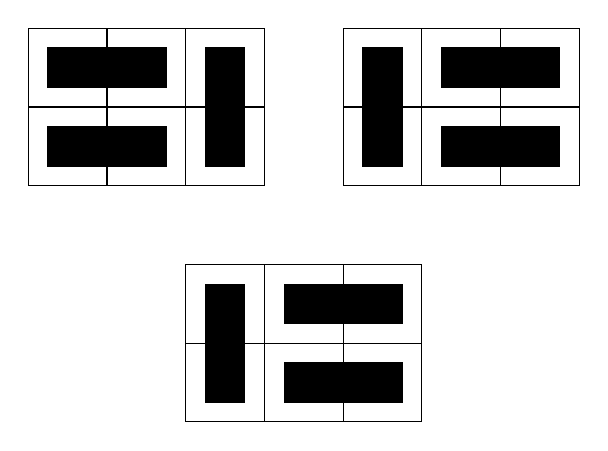
\begin{tikzpicture}[x=1.0cm, y=1.0cm]
        \foreach \y in {0,1} {
            \foreach \x in {0,1,2} {
                \draw (0+\x ,0+\y) rectangle ++ (1,1);
            }
        }

        \draw[fill, black] (0.25 ,0.25) rectangle ++ (1.5,0.5);
        \draw[fill, black] (0.25 ,1.25) rectangle ++ (1.5,0.5);
        \draw[fill, black] (2.25 ,0.25) rectangle ++ (0.5,1.5);

        \foreach \y in {0,1} {
            \foreach \x in {0,1,2} {
                \draw (4+\x ,0+\y) rectangle ++ (1,1);
            }
        }

        \draw[fill, black] (4+1.25 ,0.25) rectangle ++ (1.5,0.5);
        \draw[fill, black] (4+1.25 ,1.25) rectangle ++ (1.5,0.5);
        \draw[fill, black] (4+0.25 ,0.25) rectangle ++ (0.5,1.5);

        \foreach \y in {0,1} {
            \foreach \x in {0,1,2} {
                \draw (2+\x ,-3+\y) rectangle ++ (1,1);
            }
        }

        \draw[fill, black] (2+1.25 ,-3+0.25) rectangle ++ (1.5,0.5);
        \draw[fill, black] (2+1.25 ,-3+1.25) rectangle ++ (1.5,0.5);
        \draw[fill, black] (2+0.25 ,-3+0.25) rectangle ++ (0.5,1.5);
    \end{tikzpicture}
\end{center}
好的,再看一种情况,当 $n=4$ 时,我们看到 $T(4)=5$。

\begin{center}
    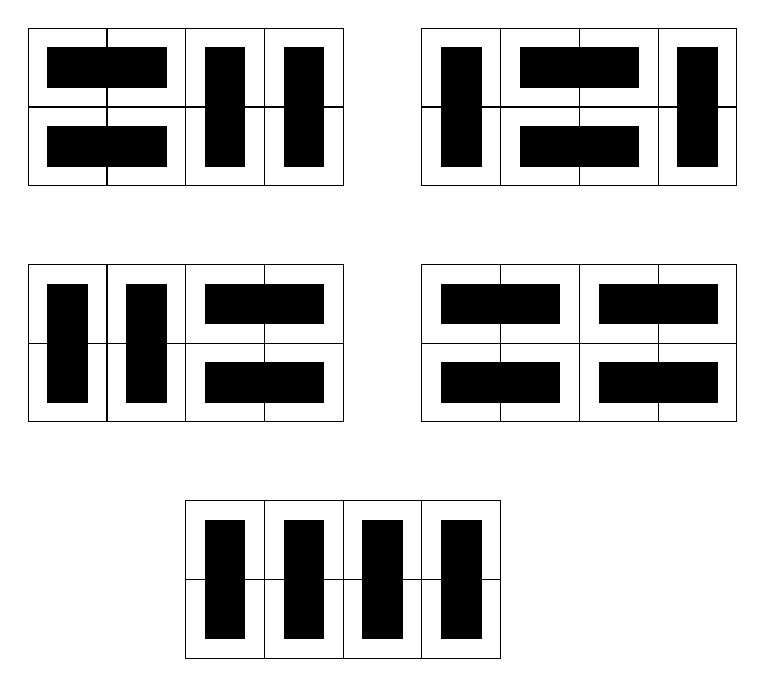
\begin{tikzpicture}[x=1.0cm, y=1.0cm]
        \foreach \y in {0,1} {
            \foreach \x in {0,...,3} {
                \draw (0+\x ,0+\y) rectangle ++ (1,1);
            }
        }

        \draw[fill, black] (0.25 ,0.25) rectangle ++ (1.5,0.5);
        \draw[fill, black] (0.25 ,1.25) rectangle ++ (1.5,0.5);
        \draw[fill, black] (2.25 ,0.25) rectangle ++ (0.5,1.5);
        \draw[fill, black] (3.25 ,0.25) rectangle ++ (0.5,1.5);

        \foreach \y in {0,1} {
            \foreach \x in {0,...,3} {
                \draw (5+\x ,0+\y) rectangle ++ (1,1);
            }
        }

        \draw[fill, black] (5+1.25 ,0.25) rectangle ++ (1.5,0.5);
        \draw[fill, black] (5+1.25 ,1.25) rectangle ++ (1.5,0.5);
        \draw[fill, black] (5+0.25 ,0.25) rectangle ++ (0.5,1.5);
        \draw[fill, black] (5+3.25 ,0.25) rectangle ++ (0.5,1.5);

        \foreach \y in {0,1} {
            \foreach \x in {0,...,3} {
                \draw (0+\x ,-3+\y) rectangle ++ (1,1);
            }
        }

        \draw[fill, black] (2.25 ,-3+0.25) rectangle ++ (1.5,0.5);
        \draw[fill, black] (2.25 ,-3+1.25) rectangle ++ (1.5,0.5);
        \draw[fill, black] (0.25 ,-3+0.25) rectangle ++ (0.5,1.5);
        \draw[fill, black] (1.25 ,-3+0.25) rectangle ++ (0.5,1.5);

        \foreach \y in {0,1} {
            \foreach \x in {0,...,3} {
                \draw (5+\x ,-3+\y) rectangle ++ (1,1);
            }
        }

        \draw[fill, black] (5+2.25 ,-3+0.25) rectangle ++ (1.5,0.5);
        \draw[fill, black] (5+2.25 ,-3+1.25) rectangle ++ (1.5,0.5);
        \draw[fill, black] (5+0.25 ,-3+0.25) rectangle ++ (1.5,0.5);
        \draw[fill, black] (5+0.25 ,-3+1.25) rectangle ++ (1.5,0.5);

        \foreach \y in {0,1} {
            \foreach \x in {0,...,3} {
                \draw (2+\x ,-6+\y) rectangle ++ (1,1);
            }
        }

        \draw[fill, black] (2+0.25 ,-6+0.25) rectangle ++ (0.5,1.5);
        \draw[fill, black] (2+1.25 ,-6+0.25) rectangle ++ (0.5,1.5);
        \draw[fill, black] (2+2.25 ,-6+0.25) rectangle ++ (0.5,1.5);
        \draw[fill, black] (2+3.25 ,-6+0.25) rectangle ++ (0.5,1.5);
    \end{tikzpicture}
\end{center}

我们现在可以开始寻找模式了吗?找到更大棋盘的密铺会很繁琐!让我们考虑一下如何利用 $T(1) = 1$ 的事实来推断出有关 $T(2)$ 的信息……等一下……做不到,对吧?这两个案例有本质的区别。具体来说,由于多米诺骨牌的大小为 $2 \times 1$,因此我们仅向棋盘中添加一行这一事实对我们没有帮助。

好吧,那么我们考虑 $n = 3$。我们可以利用 $T(2) = 2$ 这个事实吗?在这种情况下,答案是肯定的!知道 $2 \times 2$ 棋盘有两个密铺,无需太多思考,我们可以立即构建 $2 \times 3$ 棋盘的两个平铺。具体来说,我们可以将\emph{垂直多米诺骨牌添加}到之前的每一个密铺中。但我们知道 $T(3) = 3$。第三个密铺从何而来?再次查看该密铺,以及它与其他两个密铺的比较。在第三个密铺中,右侧的多米诺骨牌是水平的,而不是其他两种密铺中的垂直多米诺骨牌。如果我们移除这两个平行的水平多米诺骨牌,我们就会得到 $n = 1$ 时的情况。换句话说,我们可以通过在右侧\emph{添加一个由两个水平多米诺骨牌组成的正方形}来构建 $2 \times 3$ 棋盘的密铺。总的来说,我们已经用较小尺寸的棋盘(即 $2 \times 2$ 和 $2 \times 1$)描述了 $2 \times 3$ 棋盘的所有密铺:

\begin{center}
    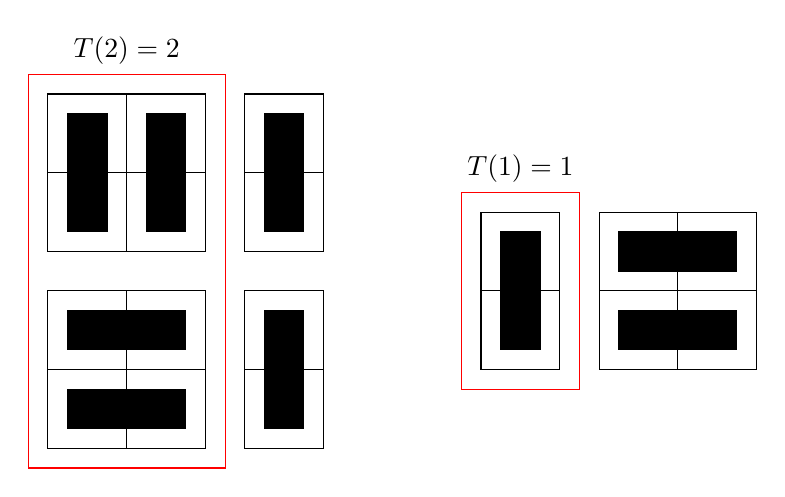
\begin{tikzpicture}[x=1.0cm, y=1.0cm]
        \foreach \g in {0, 2.5} {
            \foreach \y in {0,1} {
                \foreach \x in {0,1} {
                    \draw (0+\x ,0+\y+\g) rectangle ++ (1,1);
                }
            }
            \draw (2.5,0+\g) rectangle ++ (1,1);
            \draw (2.5,1+\g) rectangle ++ (1,1);
            \draw[fill, black] (2.75 ,0.25+\g) rectangle ++ (0.5,1.5);
        }

        \draw[fill, black] (0.25 ,0.25) rectangle ++ (1.5,0.5);
        \draw[fill, black] (0.25 ,1.25) rectangle ++ (1.5,0.5);

        \draw[fill, black] (0.25 ,2.5+0.25) rectangle ++ (0.5,1.5);
        \draw[fill, black] (1.25 ,2.5+0.25) rectangle ++ (0.5,1.5);

        \draw[red] (-0.25, -0.25) rectangle ++(2.5, 5);
        \path (-0.25,4.75) --  (2.25,4.75) node[midway,above,black] {$T(2)=2$};

        \draw (5.5,1) rectangle ++ (1,1);
        \draw (5.5,2) rectangle ++ (1,1);
        \draw[fill, black] (5.75 ,1.25) rectangle ++ (0.5,1.5);
        \draw[red] (5.25, 0.75) rectangle ++(1.5, 2.5);
        \path (5.25,3.25) --  (6.75,3.25) node[midway,above,black] {$T(1)=1$};

        \foreach \y in {0,1} {
            \foreach \x in {0,1} {
                \draw (7+\x ,1+\y) rectangle ++ (1,1);
            }
        }
        \draw[fill, black] (7.25 ,1.25) rectangle ++ (1.5,0.5);
        \draw[fill, black] (7.25 ,2.25) rectangle ++ (1.5,0.5);

    \end{tikzpicture}
\end{center}
\[T(3) = 3 = 2 + 1 = T(2) + T(1)\]

现在你可能会看出模式来!我们再看一下当 $n = 4$ 时会发生什么,我们将垂直多米诺骨牌添加到构成 $T(3)$ 的每一个密铺中,或者将两个水平多米诺骨牌添加到构成 $T(2)$ 的每一个密铺中,以此得到 $T(4)$ 的\emph{所有}密铺:

\begin{center}
    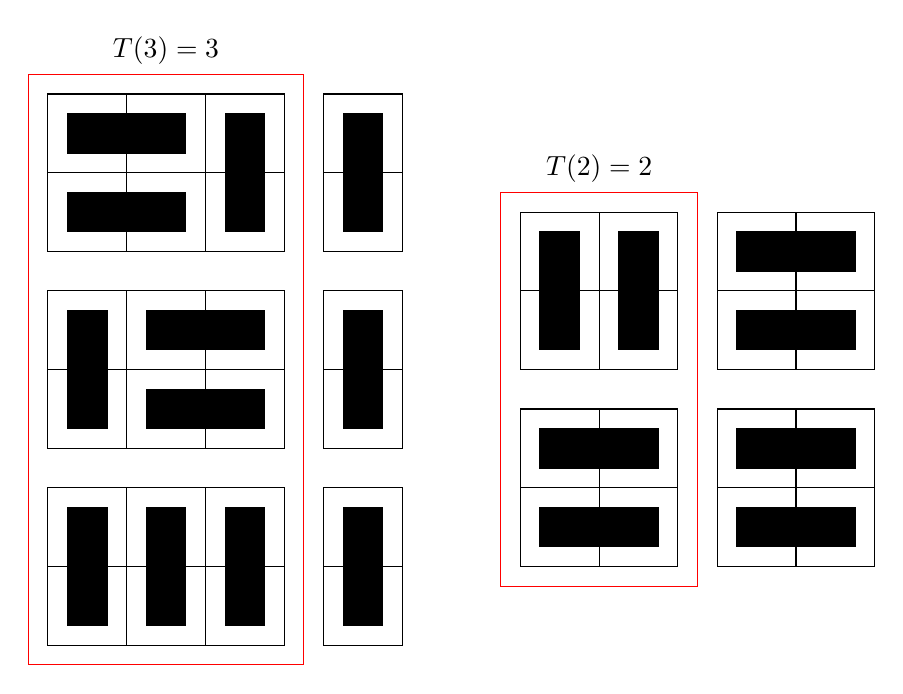
\begin{tikzpicture}[x=1.0cm, y=1.0cm]
        \foreach \g in {0, 2.5, 5} {
            \foreach \y in {0,1} {
                \foreach \x in {0,1,2} {
                    \draw (0+\x ,0+\y+\g) rectangle ++ (1,1);
                }
            }

            \draw (3.5,\g+0) rectangle ++ (1,1);
            \draw (3.5,\g+1) rectangle ++ (1,1);
            \draw[fill, black] (3.75 ,\g+0.25) rectangle ++ (0.5,1.5);
        }
        \draw[fill, black] (0.25 ,0.25) rectangle ++ (0.5,1.5);
        \draw[fill, black] (1.25 ,0.25) rectangle ++ (0.5,1.5);
        \draw[fill, black] (2.25 ,0.25) rectangle ++ (0.5,1.5);

        \draw[fill, black] (0.25 ,2.75) rectangle ++ (0.5,1.5);
        \draw[fill, black] (1.25 ,2.75) rectangle ++ (1.5,0.5);
        \draw[fill, black] (1.25 ,3.75) rectangle ++ (1.5,0.5);

        \draw[fill, black] (2.25 ,5.25) rectangle ++ (0.5,1.5);
        \draw[fill, black] (0.25 ,5.25) rectangle ++ (1.5,0.5);
        \draw[fill, black] (0.25 ,6.25) rectangle ++ (1.5,0.5);

        \draw[red] (-0.25, -0.25) rectangle ++(3.5, 7.5);
        \path (-0.25,7.25) --  (3.25,7.25) node[midway,above,black] {$T(3)=3$};


        \foreach \g in {0, 2.5} {
            \foreach \y in {0,1} {
                \foreach \x in {0,1} {
                    \draw (6+\x ,1+\y+\g) rectangle ++ (1,1);
                }
            }
            \foreach \y in {0,1} {
                \foreach \x in {0,1} {
                    \draw (8.5+\x ,1+\y+\g) rectangle ++ (1,1);
                }
                \draw[fill, black] (8.75 ,1.25+\g+\y) rectangle ++ (1.5,0.5);
            }
           
        }

        \draw[fill, black] (6.25 ,1.25) rectangle ++ (1.5,0.5);
        \draw[fill, black] (6.25 ,2.25) rectangle ++ (1.5,0.5);

        \draw[fill, black] (6.25 ,3.5+0.25) rectangle ++ (0.5,1.5);
        \draw[fill, black] (7.25 ,3.5+0.25) rectangle ++ (0.5,1.5);

        \draw[red] (5.75, 0.75) rectangle ++(2.5, 5);
        \path (5.75,5.75) --  (8.25,5.75) node[midway,above,black] {$T(2)=2$};
        
    \end{tikzpicture}
\end{center}
\[T(4) = 5 = 3 + 2 = T(3) + T(2)\]

另请注意,用这种方式不会产生重复的 $2 \times 4$ 密铺。(仔细想想为什么会这样。我们用一种什么方法表征两种密铺可以保证它们不重复?)有了这些信息,我们可以立即得出结论 $T(4) = T(3) + T(2)$。

此外,我们可以概括这样一个论点;$n = 4$ 没有什么特别的,对吧?对于任意特定的 $n$,我们可以只考虑所有可能的密铺,然后看看棋盘\emph{最右侧}发生的情况:要么有一个垂直多米诺骨牌(这意味着密铺来自 $2 \times (n - 1)$ 棋盘),要么有两个水平多米诺骨牌(这意味着密铺来自 $2 \times (n-2)$ 棋盘)。有了这个论点的支撑,对于所有有意义的 $n$ 值,我们可以得出如下结论:
\[T(n) = T(n - 1) + T(n - 2)\]
哪些 $n$ 值有意义?请记住,我们必须单独分析 $T(1)$ 和 $T(2)$;因此这个论点不适用于 $n=1$ 和 $n=2$,我们必须添加限制条件 $n \ge 3$ 才能使上面公式成立。

有了这些信息,只要有足够的时间,我们就可以轻松计算出任意 $n$ 值下的 $T(n)$。我们甚至可以相当容易地编写出计算机程序。然而,正是这种\emph{归纳}论证——我们注意到的模式以及我们对其发生原因的彻底描述——让我们首先得出了结论。这种情况下,每一项的值 $T(n)$ 取决于前\emph{两}项 $T(n-1)$ 和 $T(n-2)$ 的值。这在本章之前的例子中\emph{没有}出现过,它暗示了这里发生了更深层次的事情。你是否发现我们之前对归纳的定义以及多米诺骨牌的类比在这里不再适用?你会如何修正我们的类比来解释这种情况?思考一下这些问题,然后继续阅读。我们将在下一个示例之后更深入地讨论它们。

顺便一提,你是否注意到此示例的解有一些有趣的地方?你还知道其他类似的数列吗?想一想……


% !TeX root = ../../../book.tex
\subsection{制胜策略}

这个例子将是我们第一个\emph{无需}证明数值公式的归纳问题!这似乎有些奇怪,但正如即将看到的,事实确实如此。实际上在数学中,这种情况比你想象的更为常见:一个问题或数学对象可能蕴含潜在的归纳结构,却并不依赖代数或算术的具体内容。

具体来说,我们将讨论一个\emph{游戏}。它是通常意义上的游戏——有玩家必须遵守的规则以及明确的胜负判定——同时也是数学意义上的游戏:我们可以用数学符号精确描述规则和情境,并抽象地探讨\emph{策略},甚至能\emph{解}出这个游戏。这与棒球比赛截然不同。

现在介绍游戏规则,我们暂且称之为``取石子''。有两名玩家 $P_1$ 和 $P_2$,$P_1$ 先行。桌上有两堆石子,每堆恰好有 $n$ 个($n$ 为自然数)。为区分不同版本,当每堆石子数为 $n$ 时,我们称玩家在进行``$T_n$ 游戏''。每回合玩家可从\emph{任意}一堆取走\emph{任意}数量的石子(不可同时取两堆)。取走\emph{最后}一颗石子者\emph{获胜}。

试着跟朋友玩一下这个游戏。用硬币或糖果代替石子,并试着互换 $P_1$/$P_2$ 角色。尝试制定获胜\emph{策略}——最大化胜率的玩法,推测不同 $n$ 值下的胜负关系。谁``应该''获胜?能否给出\emph{证明}?请务必先亲自体验游戏并尝试给出证明,再继续阅读我们的分析。你可能会惊讶于自己的发现!

与其他示例一样,我们先观察 $n$ 为较小数值的情形再进行推广。当 $n = 1$ 时,游戏很简单:$P_1$ 只能取走其中一堆的唯一石子,随后 $P_2$ 取走另一堆的石子获胜。(注意:无论 $P_1$ 选择哪堆,$P_2$ 总能取走剩余的石子。我们可以说``不失一般性'',假设 $P_1$ 选左堆,因为两堆等价。后文讨论数理逻辑时,我们将深入探讨``不失一般性''这一概念。)

\begin{center}
    \begin{tikzpicture}[line width=0.5mm]
        \foreach \n in {0, 1}{
            \node at (\n, 0)[circle,fill,inner sep=8pt, anchor=west]{};
            \draw (\n, -1) -- +(0.8, 0);
        }
        \draw[-latex] (2.5, -0.4) -- +(2, 0) node[midway,above]{$P_1$ 回合};
        \draw (5, -1) -- +(0.8, 0);
        \node at (6, 0)[circle,fill,inner sep=8pt, anchor=west]{};
        \draw (6, -1) -- +(0.8, 0);
        \draw[-latex] (7.5, -0.4) -- +(2, 0) node[midway,above]{$P_2$ 回合};
        \draw (10, -1) -- +(0.8, 0);
        \draw (11, -1) -- +(0.8, 0);
        \path (10, -0.4) -- +(2, 0) node[midway,above]{$P_2$ 胜!};
    \end{tikzpicture}
\end{center}

当 $n = 2$ 时,可能出现几种情况。考虑玩家 $P_1$ 可能的行动。虽然 $P_1$ 可选择左堆或右堆,但由于最终结果相同且两堆可交换,不妨设(不失一般性)$P_1$ 从左堆取走若干石子。具体而言,可能取一颗或两颗石子。下面对每种情况分别讨论。

\begin{center}
    \begin{tikzpicture}[line width=0.5mm]
        \foreach \x in {0, 1}{
            \node at (\x, 0)[circle,fill,inner sep=8pt, anchor=west]{};
            \node at (\x, 1)[circle,fill,inner sep=8pt, anchor=west]{};
            \draw (\x, -1) -- +(0.8, 0);
        }
        \draw[-latex] (2.5, -0.4) -- +(2, -0.6);
        \draw[-latex] (2.5, 0.6) -- +(2, 0.6);
        \node[anchor=west] at(2.5,0) {$P_1$ 回合};
        \foreach \delta in {1, -2}{
            \foreach \n in {0, 1}{
                \draw (5+\n, \delta) -- +(0.8, 0);
                \node at (6, \delta+1+\n)[circle,fill,inner sep=8pt, anchor=west]{};
            }
        }
        \node at (5, -1)[circle,fill,inner sep=8pt, anchor=west]{};
        \draw[-latex] (7.5, 2) -- +(2, 0) node[midway,above]{$P_2$ 回合};
        \draw[-latex] (7.5, -1) -- +(2, 0) node[midway,above]{$P_2$ 回合};
        \draw (10, 1) -- +(0.8, 0);
        \draw (11, 1) -- +(0.8, 0);
        \path (10, 1.6) -- +(2, 0) node[midway,above]{$P_2$ 胜!};
        \path (10, -1.4) -- +(2, 0) node[midway,above]{???};
    \end{tikzpicture}
\end{center}

若 $P_1$ 取走两颗石子,$P_2$ 应该如何应对?此时 $P_2$ 可以取走另一堆的全部石子从而获胜,因此 $P_1$ 不应采取此行动。但为全面分析游戏,仍需考虑所有可能情况。故在此情形下(对应示意图上半部分),$P_2$ 获胜。此情况较为简单。

若 $P_1$ 仅从左堆取走一颗石子(对应示意图下半部分),$P_2$ 应该如何应对?此时存在多种选择:

\begin{itemize}
    \item 若 $P_2$ 从左堆取走最后一颗石子,则 $P_1$ 可以取走右堆全部石子获胜。
    \item 若 $P_2$ 从右堆取走全部两颗石子,则 $P_1$ 可以取走左堆最后一颗石子获胜。
    \item 若 $P_2$ 仅从右堆取走一颗石子……
\end{itemize}

\begin{center}
    \begin{tikzpicture}[line width=0.5mm]
        \foreach \g in {0, 5, 10} {
            \foreach \x in {0, 1} {
                \node at (\x+\g, 0)[circle,fill,inner sep=8pt, anchor=west]{};
                \draw (\x+\g, -1) -- +(0.8, 0);
            }
        }
        \node at (0, 1)[circle,fill,inner sep=8pt, anchor=west]{};
        \node at (1, 1)[circle,fill,inner sep=8pt, anchor=west]{};
        \draw[-latex] (2.5, -0.4) -- +(2, 0) node[midway,above]{$P_1$ 回合};

        \node at (6, 1)[circle,fill,inner sep=8pt, anchor=west]{};
        \draw[-latex] (7.5, -0.4) -- +(2, 0) node[midway,above]{$P_2$ 回合};
    \end{tikzpicture}
\end{center}

此时局面与 $T_1$ 完全相同,而该情形已分析过:由于此时轮到 $P_1$ 行动,无论其如何操作,$P_2$ 都将获胜。对 $P_2$ 而言,此乃最优应对——\emph{无论} $P_1$ \emph{采取何种行动},$P_2$ 均可获胜!

综上可见:无论 $P_1$ 初始采取何种行动(从任意堆取一或两颗石子),$P_2$ 总能作出\emph{特定回应以保证获胜},且此后无论 $P_1$ 如何应对均无法改变结果。$P_2$ 已占据不败之地。现在让我们进一步探究其他 $n$ 值的情形。

当 $n = 3$ 时,我们再次不失一般性地假设玩家 $P_1$ 首先从左侧石子堆取石子。他可以取走一颗、两颗或三颗石子:
\begin{itemize}
    \item 若 $P_1$ 取走全部三颗石子,则 $P_2$ 将直接取走另一堆石子并获胜。
    \item 若 $P_1$ 取走两颗石子……此时 $P_2$ 应该如何应对?
\end{itemize}
$P_2$ 若取空右侧堆是愚蠢的($P_1$ 随后可取空左侧堆获胜),同样取空左侧堆也不明智($P_1$ 可以立即取空右侧堆获胜),因此需采取折中策略。若 $P_2$ 仅从右侧堆取走一颗石子,$P_1$ 可采取相同策略回应,导致两堆均剩一颗石子且轮次互换——此时 $P_2$ 成为先手方。根据此前分析,$P_2$ 在此局面下必败,因此这是一个糟糕的策略!

\begin{center}
    \begin{tikzpicture}[line width=0.5mm]
        \foreach \g in {0, 5, 10, 15}{
            \foreach \x in {0, 1}{
                \node at (\x+\g, 0)[circle,fill,inner sep=8pt, anchor=west]{};
                \draw (\x+\g, -1) -- +(0.8, 0);
            }
        }
        \foreach \x in {0, 1, 6}{
            \foreach \y in {0, 1}{
                \node at (\x, \y)[circle,fill,inner sep=8pt, anchor=west]{};
                \node at (\x, \y+1)[circle,fill,inner sep=8pt, anchor=west]{};
            }
        }

        \node at (11, 1)[circle,fill,inner sep=8pt, anchor=west]{};

        \draw[-latex] (2.5, -0.4) -- +(2, 0) node[midway,above]{$P_1$ 回合};
        \draw[-latex] (7.5, -0.4) -- +(2, 0) node[midway,above]{$P_2$ 回合};
        \draw[-latex] (12.5, -0.4) -- +(2, 0) node[midway,above]{$P_1$ 回合};
        \path (15, 0.6) -- +(2, 0) node[midway,above]{$P_1$ 胜!};
    \end{tikzpicture}
\end{center}

让我们重新推演:若 $P_2$ 从右侧堆取走两颗石子……局面立现转机!此时每堆仅余一颗石子,$P_1$ 作为先手必败,$P_2$ 锁定胜局!

\begin{center}
    \begin{tikzpicture}[line width=0.5mm]
        \foreach \g in {0, 5, 10}{
            \foreach \x in {0, 1}{
                \node at (\x+\g, 0)[circle,fill,inner sep=8pt, anchor=west]{};
                \draw (\x+\g, -1) -- +(0.8, 0);
            }
        }
        \foreach \x in {0, 1, 6}{
            \foreach \y in {0, 1}{
                \node at (\x, \y)[circle,fill,inner sep=8pt, anchor=west]{};
            }
        }
        \draw[-latex] (2.5, -0.4) -- +(2, 0) node[midway,above]{$P_1$ 回合};
        \draw[-latex] (7.5, -0.4) -- +(2, 0) node[midway,above]{$P_2$ 回合};
        \path (10, 0.6) -- +(2, 0) node[midway,above]{$P_2$ 胜!};
    \end{tikzpicture}
\end{center}

考虑 $n = 4$ 的情形,类似分析依然适用。玩家 $P_1$ 可以从左侧堆取走一至四颗石子。但无论其如何操作,$P_2$ 皆可在另一堆上\emph{模仿}相同动作,将游戏简化为更小规模的已知局面,从而确保胜利!$P_2$ 似乎始终占据主动:他能通过镜像策略回应 $P_1$ 的任何操作。无论 $P_1$ 采取何种行动,$P_2$ 的针对性回应终将导向胜利。因此我们称``$P_2$ 拥有必胜策略''——其具备明确的方法评估局势并选择特定行动以\emph{确保获胜}。

我们要如何证明这一点?如何运用本章的归纳法?目前或许难以窥见全貌。我们究竟需要证明什么?此处的多米诺骨牌或阶梯类比如何具象化?思考这个案例时需领悟:归纳法不仅关乎代数表达式,更体现某种``递推''结构,即大规模情形依赖于小规模情形;我们需先证明初始事实,再论证如何将任意更大规模情形化归为已证事实。这才是多米诺类比的本质。该类比虽能有效阐释部分归纳问题(非全部)且具有直观感染力,但并非普适于\emph{所有}场景。

回顾本章给出的四个案例,辨析其异同。尝试用更精准的数学语言(或自创术语)描述数学归纳法(需超越直观类比)。令人惊叹的是,即使尚未掌握``标准''表述,但你仍能通过此过程深化理解并获得精妙描述!后续我们将严格陈述并证明数学归纳法及其变体。在此之前,需先探索其他数学领域以构建必要的语言、符号与知识基础。不过启程之前,不妨先了解一下数学归纳法的若干经典应用。


% !TeX root = ../../../book.tex
\subsection{习题}

\subsubsection*{温故知新}

以口头或书面的形式简要回答以下问题。这些问题全都基于你刚刚阅读的内容,所以如果忘记了具体的定义、概念或示例,可以回去重读相关部分。确保在继续学习之前能够自信地回答这些问题,这将有助于你的理解和记忆!

\begin{enumerate}[label=(\arabic*)]
    \item 这两个例子如何\emph{归纳}?它们在哪些方面与前面的例子(立方体和直线)相似?哪些方面有所不同?
    \item 对于多米诺骨牌密铺问题,我们需要知道多少个先前值才能计算 $T(n)$?
    \item $T(n) = T(n - 1) + T(n - 2)$ 和 $T(n + 2) = T(n + 1) + T(n)$ 有什么区别?
    \item 取石子游戏的必胜策略是什么?尝试与一个不了解该游戏的朋友一起玩一下,并使用玩家 $P_2$ 的必胜策略。每次你都获胜时他们有多沮丧?他们也开始发现这个策略了吗?
\end{enumerate}

\subsubsection*{小试牛刀}

尝试回答以下问题。这些题目要求你实际动笔写下答案,或(对朋友/同学)口头陈述答案。目的是帮助你练习使用新的概念、定义和符号。题目都比较简单,确保能够解决这些问题将对你大有帮助!

\begin{enumerate}[label=(\arabic*)]
    \item $T(5)$ 会是怎样?你能画出所有密铺方案吗?
    \item 探讨用两堆各 $4$ 颗石子进行取石子游戏的可能性。你能确保玩家 $P_2$ 总是有必胜策略吗?
    \item \textbf{挑战题:}如果用\emph{三堆}相同大小的石子来玩``取石子''游戏,会发生什么?你能为任意一方找到获胜策略吗?尝试和朋友一起玩一下,看看会发生什么!
    \item 查看\emph{斐波那契数列}。它与我们在多米诺骨牌密铺示例中发现的数列 $T(n)$ 有什么关系?
\end{enumerate}

\newpage
% !TeX root = ../../../book.tex
\section{应用}

% !TeX root = ../../../book.tex
\subsection{递归程序}\label{sec:section2.5.1}

数学归纳法背后的概念也大量应用于计算机科学中。回想一下我们当初是如何推导出 $\sum_{k=1}^{n}k^2$ 的公式的。一旦我们找到了用更小的立方和剩余项来表示立方数的方法,我们就会一遍又一遍地重复这个替代过程,直到我们到达``最简单''的情况,即我们在开始计算问题:$2^3=1+3+3+1$ 时第一次观察到的情况。递归编程利用了这一技术:为了解决``大''问题,确定问题如何依赖于``小''案例,并化简问题,直到达到一个简单的已知案例。

此类技术的一个经典示例是编写代码来计算\emph{阶乘} $n!$,它被定义为前 $n$ 个自然数的乘积:
\[n! = 1 \cdot 2 \cdot 3 \dots (n - 1) \cdot n\]
这是一个简单的定义,我们作为人类可以直观地理解,但告诉计算机如何执行该产品的方式并不完全相同。(尝试一下!怎么用计算机代码表达``继续执行,直到达到 $n$''?)事实上,对函数进行编程的一种更有效的方法,以及对数学归纳定义进行建模的方法,是让一个程序\emph{递归地调用自身},直到达到``最简''情况。在阶乘种,这种情况就是 $1! = 1$。对于 $n$ 的任意其他值,我们可以简单地不断应用以下知识:
\[n! = (n - 1)! \cdot n\]
来计算 $n!$。下面的\emph{伪代码}描述了这一思想:

\begin{verbatim}
    factorial(n):
        if n = 1
            return 1
        else
            return n * factorial(n-1)
    end
\end{verbatim}

我们知道 $1! = 1$,因此如果要求程序计算该值,则会立即返回正确的结果。对于任意大于 $1$ 的 $n$ 值,程序都会引用\emph{自身},并说:``为我计算 $(n-1)!$,然后我在后面乘上 $n$ 就得到答案了。''为了计算 $(n-1)!$,程序会再次询问输入是否为 $1$;如果不为 $1$,则会继续调用自身并说:``为我计算 $(n-2)!$,然后我在后面乘上 $(n-1)$ 。'' 这个过程一直持续到程序返回 $1! = 1$。从那之后,程序就知道如何求出 $2! = 1 \times 2$,然后是 $3! = 2! \times 3$,依此类推,直到 $n! = (n - 1)! \times n$。

递归编程的另一个经典例子是\emph{斐波那契数}。可能你之前在数学课上见过这个数列。(事实上,我们在上一节多米诺骨牌密铺中提到过该数列!)你可能还听说过斐波那契数列以一些有趣和奇怪的方式出现在自然界中。(该数列最早是由比萨的意大利数学家莱昂纳多·斐波那契(Leonardo Fibonacci)在研究兔子种群增长时``发现''的。)斐波那契数列的前两项均为 $1$,数列中的任意数字都被定义为前两个数字之和。也就是说,如果我们用 $F(n)$ 表示第 $n$ 个斐波那契数,那么
\[F(1) = 1 \text{ 且 }F(2) = 1, \text{ 对于任意 } n \ge 3, F(n) = F(n - 1) + F(n - 2)\]
那么,$F(5)$ 等于多少?$F(100)$ 呢?$F(10000)$ 呢?这可以通过递归程序很容易地处理。思路是一样的:如果程序遇到``简单情况''之一,即 $F(1)$ 或 $F(2)$,则立即返回正确值 $1$。否则,将调用自身来计算前两个数字,然后将它们相加。阅读下面的伪代码并思考它是如何工作的。如果我们使用这个程序来计算 $F(10)$ 会发生什么?怎样才能得出答案呢?

\begin{verbatim}
    Fibonacci(n):
        if n = 1 or n = 2
            return 1
        else
            return Fibonacci(n-1) + Fibonacci(n-2)
    end
\end{verbatim}

上面程序与 \verb|factorial| 程序的思路相同(让程序调用自身来计算函数``较小''情况的值,直到达到已知值),但这里有一些更深层次的内容。但这里有一些更深层次的内容。如果我们将 $n = 10$ 输入到程序中,它会识别出还不知道应该输出什么值,于是会调用自身来计算 \verb|Fibonacci(9)| 和 \verb|Fibonacci(8)|。对程序的每次调用,都会再次识别出该值未知。因此,会再次调用自身来计算 \verb|Fibonacci(8)| 和 \verb|Fibonacci(7)|,以及 \verb|Fibonacci(7)| 和 \verb|Fibonacci(6)|。没错,程序使用相同的输入值多次调用自身。为了计算 $F(9)$,我们需要知道 $F(8)$ 和 $F(7)$,但同时,为了计算 $F(8)$,我们还需要知道 $F(7) $ 和 $F(6)$。这样,我们最终多次调用程序 \verb|Fibonacci|。

尝试比较 \verb|Fibonacci| 程序和 \verb|factorial| 程序,特别是关于我们在本章中研究的归纳过程。他们使用类似的思路吗? 它们与我们介绍数学归纳法时用到的``多米诺骨牌''类比有何关系?将多米诺骨牌 $n$ 上的``事实''视为对 $n!$ 的正确计算或 $F(n)$。这个类比在每种情况下如何发挥作用?所有多米诺骨牌都会倒下吗?在你继续阅读时,请记住这些问题。所有这些想法背后都有一些非常强大的数学基础。

\clearpage


% !TeX root = ../../../book.tex
\subsection{汉诺塔}

我们稍作休息来玩个游戏吧。虽然严格来说不算完全放松——因为它本质上是关于\emph{归纳}的练习,所以与主题密切相关——但至少是个游戏!\emph{汉诺塔}作为经典智力游戏广受欢迎,部分得益于其简洁的规则和道具。然而它的解法可绝不简单!

假设有三根垂直立柱,以及三个大小不同的圆盘(\textcolor{blue}{蓝色}、\textcolor{olivegreen}{绿色}、\textcolor{red}{红色})叠放其中,初始状态如下:
\begin{center}
    \begin{tikzpicture}[line width=4mm,line cap=round,xscale=3,brown!30]
        \def\sequence{3/1,2/1,1/1}
        % init colors
        \foreach[count=\j] \c in {red,olivegreen,blue}
            \gset col[\j]={\c};
        \edef\numdisks{\j}
        % init positions and draw support
        \foreach \j in {1,2,3}{
            \gset pos[\j]=0
            \draw (\j,-.4) -- +(0,3);
        }
        \draw (.5,-.4) -- +(3,0);

        % draw
        \foreach[count=\k] \i/\j in \sequence{
            \edef\delta{\i*0.4/3}
            \draw[draw={\get col[\i]}](\j-\delta,\get pos[\j]) -- (\j+\delta,\get pos[\j]);
            \ginc pos[\j]+={.4}
        }
    \end{tikzpicture}
\end{center}
目标是将所有圆盘移至另一立柱(左中右皆可),但需遵守两条规则:
\begin{enumerate}
    \item 每次只能移动一个圆盘,且必须从某立柱顶端移至另一立柱顶端;
    \item 任何圆盘不可置于比它小的圆盘之上。
\end{enumerate}
规则虽简,破解却难!建议用硬币或扑克牌模拟(亦可购买专用套件)。你能破解这个问题吗?用了多少步?这是最优解吗?原因何在?

既然这是归纳游戏,我们深入探究:解决此谜题需多少步?(一步指单个圆盘的移动)更关键的是,如何确定\emph{最小步数}?以三个圆盘为例,若反复移动最小圆盘 $100$ 次后再求解,显然非最优。那么如何证明某种解法的步数已达最小值?

为了解决这个问题,我们将尝试\emph{递归分解}解法。此过程能回答更一般的问题:$n$ 个圆盘在三柱汉诺塔中的最小移动步数是多少?以 $3$ 个圆盘引入是为了便于理解,但通过深入分析可解决一般情况。为确保理解一致,先演示 $3$ 个圆盘的解法:

\begin{center}
    \begin{tikzpicture}[line width=2.6mm,line cap=round,xscale=1.5,yscale=0.5,brown!30]
        \def\sequencelist{{3/1,2/1,1/1}, {3/1,2/1,1/3}, {3/1,2/2,1/3}, {3/1,2/2,1/2}, {3/3,2/2,1/2}, {3/3,2/2,1/1}, {3/3,2/3,1/1}, {3/3,2/3,1/3}}
        % init colors
        \foreach[count=\j] \c in {red,olivegreen,blue}
            \gset col[\j]={\c};
        \edef\numdisks{\j}
        \foreach[count=\n] \sequence in \sequencelist {
            % init positions and draw support
            \foreach \j in {1,2,3}{
                \gset pos[\j]=0
                \draw (\j,-0.4-5*\n) -- +(0, 3);
            }
            \draw (0.5,-0.52-5*\n) -- +(3,0);
            % draw
            \foreach[count=\k] \i/\j in \sequence{
                \edef\delta{\i*0.4/3}
                \draw[draw={\get col[\i]}](\j-\delta,\get pos[\j]-5*\n) -- (\j+\delta,\get pos[\j]-5*\n);
                \ginc pos[\j]+={0.52}
            }
        }
        \node[black,left] at (0,-5.52){开始};
        \foreach \m in {1, ..., 7} {
            \node[black,left] at (0,-5.52-5*\m){第 \m 步};
        }   
    \end{tikzpicture}
\end{center}

请注意,最大的圆盘在多数解法中几乎是``无关紧要''的。由于我们可以在其上放置任何其他圆盘,我们只需将其他圆盘移到不同立柱上以``露出''最大圆盘,将其移至唯一的空立柱,再将其他圆盘移回即可。本质上,我们重复执行相同过程(将两个较小圆盘从一个立柱移至另一个立柱)两次,中间移动一次最大圆盘。若最大圆盘不存在,我们所做的正是解决两次 $2$ 盘问题!(仔细思考这一点,确保理解上文。可设想最大的\textcolor{blue}{蓝色}圆盘不存在,操作一遍上图的步骤。)

这表明解决 $3$ 盘问题需两次迭代解决 $2$ 盘问题,并增加一次移动最大圆盘的操作。一般而言,这揭示了问题的\emph{递归}性质:为得到 $n$ 盘问题的最优解,只需遵循解决 $(n-1)$ 盘问题的最优过程,移动一次最大的第 $n$ 个圆盘,再解决一次 $(n-1)$ 盘问题。

了解解法后,让我们确定所需步数。由于该问题需用\emph{递归}算法,任何关于最优解的\emph{证明}都需使用\emph{归纳法}。因此需要确定`起点'',即问题的``最小''或``最简''形式。对汉诺塔而言,最简形式是 $1$ 盘问题——只需一步将圆盘移至另一个立柱即可。若用 $M(n)$ 表示解决 $n$ 盘问题的最少移动次数,则 $M(1)=1$。根据前述观察:
\[\underbrace{M(2)}_{2 \text{盘问题}}= \underbrace{M(1)}_{1 \text{盘问题}}+ \underbrace{1}_{\text{移动最大圆盘}}+ \underbrace{M(1)}_{1 \text{盘问题}}= 1 + 1 + 1 = 3\]
进而可得:
\[M(3) = M(2) + 1 + M(2) = 3 + 1 + 3 = 7\]
和
\[M(4) = M(3) + 1 + M(3) = 7 + 1 + 7 = 15\]
以此类推。你发现规律了吗?这些数均为 $2$ 的幂减 $1$,即 $M(n)=2^n-1$。需指出,观察到规律不等于证明规律——它仅在前 $4$ 种情况成立,而归纳法将证明其普遍性。发现 $M(n)=2^n-1$ 本身已是重要洞见。你可以尝试求解以下递推关系:
\[M(n) = 2M(n - 1) + 1 \quad \text{且} \quad M(1) = 1\]
看看能否推导出公式 $M(n) = 2^n -1$。此闭合式优于递推式,因为 $M(n)$ 仅依赖 $n$ 而非前项(例如 $M(n-1)$)。此类关系称为\emph{递推关系},通常求解困难!

我们已知 $M(n)=2^n-1$,但验证工作留给你来完成。虽可代入数值检验,但这并非\emph{证明}。请尝试用归纳法严格证明!我们已完成了主体工作,但还需要你严谨地将一切串联在一起。请记住,你需要明确每张多米诺骨牌上的``事实''是什么,确保多米诺骨牌 $1$ 会倒下,然后对多米诺骨牌 $n$ 倒下会引起多米诺骨牌 $(n+1)$ 倒下进行一般性论证。试着写出这个证明。这些细节对你来说是否合理?向朋友展示你的证明,看看他们是否理解。你还需要向他们做出解释或指导他们完成证明阅读吗?思考最佳的解释方法与步骤,确保书面版本清晰准确。

\clearpage


% !TeX root = ../../../book.tex
\subsection{习题}

\subsubsection*{温故知新}

以口头或书面的形式简要回答以下问题。这些问题全都基于你刚刚阅读的内容,如果忘记了具体定义、概念或示例,可以回顾相关内容。确保在继续学习之前能够自信地作答这些问题,这将有助于你的理解和记忆!

\begin{enumerate}[label=(\arabic*)]
    \item 递归程序如何进行归纳?
    \item 汉诺塔的归纳结构是什么?在解决 $3$ 盘问题时,我们是如何处理 $2$ 盘问题的?
\end{enumerate}

\subsubsection*{小试牛刀}

尝试解答以下问题。这些题目需动笔书写或口头阐述答案,旨在帮助你熟练运用新概念、定义及符号。题目难度适中,确保掌握它们将大有裨益!

\begin{enumerate}[label=(\arabic*)]
    \item 根据伪代码 \verb|factorial| 的步骤计算 $5!$。
    \item 根据伪代码 \verb|Fibonacci| 的步骤计算 $F(5)$。
    \item 解决 $4$ 盘汉诺塔问题。确保你能以\emph{最优}步数 $2^4 - 1 = 15$ 步完成。
\end{enumerate}

\newpage
% !TeX root = ../../../book.tex
\section{总结}

我们已经了解了一些\textbf{归纳证明}的实例。通过解决具有相似证明模式的问题并研究不同案例,我们认识到这些证明可能涉及多样化的情境。具体而言,我们发现归纳证明\emph{并非}仅适用于求和公式或等式:它可应用于\emph{任何}依赖``先前事实''的情形。这促使我们从数学角度思考归纳法的运作机制。虽然``多米诺骨牌类比''目前是我们理解归纳法的直观方式,但接下来的核心目标是严格\emph{陈述}并\emph{证明}归纳原理。当前阶段,我们需要通过大量练习来掌握此类证明,这正是本章习题的设计目的。待后续形式化归纳法后,我们将能更熟练地运用它,并深化对这一概念的理解!

\newpage
% !TeX root = ../../../book.tex
\section{本章习题}

以下问题,有助于你熟悉归纳证明。我们暂不要求完全严格的证明,只需清晰地描述过程并写出步骤即可。待掌握数学归纳原理 (PMI) 及相应证明策略后,可重新严格证明这些问题。

\begin{exercise} \label{exc:exercises2.7.1}
    证明以下求和公式对所有自然数 $n$(包括 $n=0$)成立:
    \[\sum_{i=0}^{n}2^i=2^{n+1}-1\]
    后续问题:利用此结果说明在 $2^n$ 支球队的单场淘汰赛中,需进行多少场比赛才能决出冠军?(例如 NCAA 疯狂三月锦标赛就采用此赛制,其中 $n=6$。)
\end{exercise}

\begin{exercise}
    证明对于每个大于等于 $2$ 的自然数 $n$,均有 $3^n \ge 2^{n+1}$。
\end{exercise}

\begin{exercise}
    判断下列不等式对哪些自然数 $n$ 成立?先陈述结论,再予以证明。
    \begin{enumerate}
        \item $2^n \ge (n + 1)^2$
        \item $2^n \ge n!$
        \item $3^{n+1} > n^4$
        \item $n^3 + (n + 1)^3 > (n + 2)^3$
    \end{enumerate}
\end{exercise}

\begin{exercise}
    \textbf{末日游戏}:两名玩家轮流在日历上命名日期。每回合玩家可增加月份或日期(但不可同时增加)。从 1 月 1 日开始,说出 12 月 31 日者获胜。确定先手玩家的必胜策略。例如,以下是玩家 1 获胜的过程:
    \begin{itemize}
        \item 玩家 1: 1 月 10 日;
        \item 玩家 2: 3 月 10 日;
        \item 玩家 1: 8 月 10 日;
        \item 玩家 2: 8 月 25 日;
        \item 玩家 1: 8 月 28 日;
        \item 玩家 2: 11 月 28 日;
        \item 玩家 1: 11 月 30 日;
        \item 玩家 2: 12 月 30 日;
        \item 玩家 1: 12 月 31 日。
    \end{itemize}
    此处\emph{必胜策略}指:无论玩家 2 如何应对,玩家 1 均可依此策略\emph{保证获胜}。
\end{exercise}

\begin{exercise}
    推导并证明\emph{几何级数}求和公式。几何级数定义如下:
    \[\sum_{i=0}^{n-1}q^i\]
    其中 $q$ 为实数,$n$ 为自然数。(提示:注意 $q = 1$ 的情形。)
\end{exercise}

\begin{exercise}
    构造一个与 $n$ 相关的命题,使其对 $n=1$ 至 $n=99$ 均为真,但当 $n=100$ 时为假。
\end{exercise}

\begin{exercise}
    以下``错误证明''声称对于所有 $n$ 有 $a^n=1$,请指出其错误所在:
    \begin{spoof}
        设 $a$ 为非零实数。已知 $a^0 = 1$。我们可以归纳地写出
        \[a^{n+1} = a^n \cdot a = a^n \cdot \frac{a^n}{a^{n-1}} = 1 \cdot \frac{1}{1} = 1\]
    \end{spoof}
\end{exercise}

\begin{exercise}
    某未来社会仅流通两种硬币:$3$ Brendan 和 $8$ Brendan。法令规定,商品价格必须能用这两种硬币\textbf{精确支付}。\\
    那么一杯咖啡的合法价格可能为多少?\\
    \textbf{提示:}尝试一些较小数值并观察其中规律。
\end{exercise}

\clearpage

\begin{exercise}
    对于任意自然数 $n$,考虑大小为 $2^n \times 2^n$ 的棋盘。若移除棋盘上\textbf{任意}一个方格,能否用 L 形三格骨牌密铺剩余部分?\\
    如果答案是肯定的,请证明这一点。\\
    如果答案是否定的,请提供反例论证。(即找到一个 $n$ 值证明其不可能密铺,并解释原因。)
\end{exercise}

\begin{exercise}
    考虑一个 $n \times n$ 的正方形网格。该网格中包含多少不同大小的子方格?例如 $n=2$ 时答案为 $5$:含有 $4$ 个 $1 \times 1$ 方格和 $1$ 个 $2 \times 2$ 方格。试推导通项公式并证明其正确性。
\end{exercise}

\begin{exercise}
    证明:在不少于 $2$ 人的队列中,若队首为女性、队末为男性,则必存在某位置上一男性紧邻一女性之后。
\end{exercise}

\begin{exercise}
    证明:对于任意自然数 $n, n^3 - n$ 是 $3$ 的倍数。
\end{exercise}

\begin{exercise}
    \textbf{二进制 $n$ 元组}是由 \verb|0| 和 \verb|1| 组成的有序字符串,字符串中共有 $n$ 个数字。用\emph{归纳法}论证其总数恰为 $2^n$。
\end{exercise}

\begin{exercise}
    斐波那契数列定义为 $f_0 = 0$, $f_1 = 1$,且对于 $n \ge 2$ 有 $f_n = f_{n-1} + f_{n-2}$。这会产生序列 $0, 1, 1, 2, 3, 5, 8, 13, 21, 34, \dots$。\\
    你可能不知道,斐波那契数列也存在\emph{封闭形式};也就是说,除了上面给出的常规递归定义外,还有一个特定\emph{公式}来定义它,即:
    \[f_n = \frac{1}{\sqrt 5}\Bigg[\Bigg(\frac{1+\sqrt 5}{2}\Bigg)^n - \Bigg(\frac{1-\sqrt 5}{2}\Bigg)^n\Bigg]\]
    证明此式对所有 $n \ge 0$ 成立。
\end{exercise}

\begin{exercise}
    再次考察斐波那契数 $f_n$,证明以下结论:
    \begin{enumerate}
        \item $\displaystyle{\sum_{i=0}^{n}f_i = f_{n+2} - 1}$
        \item $\displaystyle{\sum_{i=0}^{n}f_i^2 = f_n \cdot f_{n+1}}$
        \item $\displaystyle{f_{n-1} \cdot f_{n+1} - f_n^2 = (-1)^n}$
        \item $\displaystyle{f_{m+n} = f_n \cdot f_{n+1} + f_{m-1} \cdot f_n}$
        \item $\displaystyle{f_n^2 + f_{n+1}^2 = f_{2n+1}}$
    \end{enumerate}
\end{exercise}

\begin{exercise}
    用归纳法证明:每个 $n \ge 2$ 的自然数可表为质数之积。你能证明该分解的\emph{唯一性}吗?即证明质因数分解方式\emph{只有唯一一种}。
\end{exercise}

\begin{exercise}
    证明:
    \[\sum_{k=1}^{n} k \cdot k! = 1 \cdot 1! + 2 \cdot 2! + 3 \cdot 3! + \dots + n \cdot n! = (n+1)!-1\]
\end{exercise}

\begin{exercise}
    以下``错误证明''得出所有笔颜色相同,其谬误何在?
    \begin{spoof}
        当笔数为 $1$ 时,命题显然成立。

        假设任意一组 $n$ 支笔颜色相同。(注意:我们已经解释了为什么该假设对于 $n = 1$ 成立,所以我们可以做出此假设。)取任意一组 $n + 1$ 支笔。将它们排列在桌子上,从左到右用 $1$ 到 $n + 1$ 编号。查看其中的前 $n$ 个,即查看笔 $1,2,3, \dots , n$。这是一组 $n$ 支笔,因此根据假设,该组颜色相同。(我们还不知道是什么颜色。)然后,查看最后 $n$ 支笔;即查看笔 $2,3, \dots ,n+1$。这也是一组 $n$ 支笔,因此根据假设,该组也颜色相同。而 $2$ 号笔恰好属于这两个组。因此,无论 $2$ 号笔的颜色是什么,其必然是\dotuline{两组}中每支笔的颜色。因此,所有 $n+1$ 支笔具有相同的颜色。

        根据归纳法,这表明任何一组笔,无论数量多少,都只有一种颜色。因此,纵观世界上有限数量的钢笔,我们应该只能找到一种颜色。
    \end{spoof}
\end{exercise}

\begin{exercise}
    $\star$ 本题\emph{难度极高},摘自著名数学家陶哲轩 (Terence Tao) 的博客(\href{https://terrytao.wordpress.com/2011/04/07/the-blue-eyed-islanders-puzzle-repost/}{详见链接})

    有一座小岛,岛上居住着一个部落。这个部落有 $1000$ 人,有着不同颜色的眼睛。然而,他们的宗教信仰禁止他们知道自己眼睛的颜色,甚至禁止讨论这个话题;因此,每个居民都可以(并且确实可以)看到所有其他居民眼睛的颜色,但无法知道自己眼睛的颜色(无反射物)。如果部落成员确实发现了自己眼睛的颜色,那么他们的宗教信仰就会迫使他们第二天中午在村庄广场举行自杀仪式,让所有人围观。所有的部落成员都是高度逻辑和虔诚的,他们都知道其他人也是高度逻辑和虔诚的(并且他们都知道他们都知道其他人是高度逻辑和虔诚的……)。

    (就此逻辑谜题而言,``高度逻辑的''意味着能够从岛民可用的信息和观察中逻辑推断出的任何结论,该岛民将自动知晓。)

    事实证明,在这 $1000$ 名岛民中,有 $100$ 人是蓝眼睛,$900$ 人是棕眼睛,尽管岛民最初并没有意识到这些统计数据(当然,他们每个人只能看到 $1000$ 名部落居民中的 $999$ 人)。

    一天,一名蓝眼睛的外国人来到岛上,并赢得了部落的完全信任。

    某天晚上,他向整个部落发表讲话,感谢他们的热情款待。

    然而,由于不了解当地习俗,这名外国人在讲话中提及了眼睛的颜色,他表示``\emph{在世界的其他角落看到另一个像我这样有着蓝眼睛的人是多么不同寻常啊}''。

    这种失礼(如果有的话)会给部落带来什么影响?
\end{exercise}

\newpage
% !TeX root = ../../../book.tex
\section{展望}

本章介绍了\textbf{数学归纳法}的概念。我们观察了归纳思想如何引导解题思路,并探讨了如何通过\emph{归纳证明}对此思路进行\emph{严格验证}。鉴于现有数学工具的局限,我们暂时借助非技术性类比来描述这一过程。某种程度上,这好比请朋友向从未接触过高尔夫的人解释挥杆动作:他们可提供挥杆``感受''的心理意象,但若不亲身实践,如何真正理解挥杆机制?如何学习调整动作或区分不同球杆的用法?同样,通过剖析原理与刻意练习,我们期望深入理解数学归纳法,从而能准确运用它、识别适用场景,并学会将其\emph{适配}至新情境。多米诺骨牌类比虽有助于引导直觉,但需谨记其并非数学本质。它亦无法完美解释某些案例——例如当某张骨牌的倒下不仅依赖相邻骨牌,还受之前多张骨牌影响的情形。

下一章将探讨严格表述和证明数学归纳法所需的基础概念。我们将研究\emph{数理逻辑}的相关思想,学习如何分解复杂的数学命题、如何从基础组件构建精妙的陈述,并引入新符号与简记法来压缩冗长的表述,形成简洁而精确的数学语言。在此基础上,我们将探索更基础的证明策略,并将其应用于本课程\emph{所有后续内容}——包括归纳技术本身!同时,我们还将学习\emph{集合论}的核心思想,其构成了数学各分支的基石。这不仅有助于未来系统组织思想,还能为\emph{自然数}的严格定义提供框架。掌握这两大数学分支的概念后,我们便能在坚实的基础之上构建数学归纳法,并持续正确地运用它。
